% \section{Abstract}
\begin{abstract}
The annual influenza outbreak leads to significant public health and economic burdens making it desirable to have prompt and accurate probabilistic forecasts of the disease spread. The United States Centers for Disease Control and Prevention (CDC) hosts annually a national flu forecasting competition which has led to the development of a variety of flu forecast modeling methods. For the first several years of the competition, the target to be forecast was weekly percentage of patients with an influenza-like illness (ILI), but in 2021 the target was changed to weekly hospitalization counts. Reliable state and national hospitalization data has only been available since 2021, but for ILI the data has been available since 2010 and has been successfully forecast for several seasons. % Modeling hospitalization data alone is limited to the relatively small amount of data, 
% but may be supplemented by existing ILI data which has been reported, 
% published at the state level, and successfully forecast for over a decade. 
In this manuscript, we introduce a two component modeling framework for forecasting weekly hospitalizations utilizing both hospitalization data and ILI data. The first component is for modeling ILI data using a dynamic nonlinear Bayesian hierarchical model. The second component is for modeling hospitalizations as a function of ILI. For hospitalization forecasts, ILI is first forecasted and then hospitalizations are forecast with ILI forecasts used as a linear or quadratic predictor. In a simulation study, two ILI forecast models, including one similar to the winning model for two seasons of the CDC forecast competition from \cite{osthus2019dynamic} and a nonlinear Bayesian hierarchical model from \cite{ulloa2019} are compared. Also assessed is the usefulness of including a systematic model discrepancy term in the ILI model. Forecasts of state and national hospitalizations for the 2023-24 flu season are made, and different modeling decisions are compared. We found that including a discrepancy component in the ILI model tends to improve forecasts during certain weeks of the year. We also found that other modeling decisions such as the exact nonlinear function to use in the ILI model or the error distribution for hospitalization models may or may not be better than other decisions, depending on the season, location, or week of the forecast.
% We compare hospitalization forecasts from our model to other related models submitted to the CDC forecasting competition.  


\keywords{Disease outbreak forecasting \and Bayesian hierarchical modeling \and Probabilistic forecasting \and Model discrepancy}


%\pagebreak %remove if needed

% Please include sections as the paper has, some of the following sections are meant as examples of what can be done, the bibliography should be made as given



\section{Introduction}

Every year the seasonal influenza outbreak burdens the public health system by infecting millions, causing an influx of primary care visits and hospitalizations and leading to between 290,000 and 650,000 deaths worldwide \cite[]{whoflufact2023}. \cite{molinari2007annual} estimated the United States' annual economic burden from medical costs, loss of income, and deaths to be over \$87 billion. Accurate forecasting of infectious diseases can inform public decision making and ease the burden of an outbreak \cite[]{turtle2021accurate, lutz2019applying}.
There is a growing consensus that disease forecasts should be probabilistic in nature \cite[]{gneiting2014probabilistic, bracher2021evaluating}, and it has been shown that reporting forecast uncertainty along with predictions may lead to better decision making \cite[]{ramos2013probabilistic, joslyn2012uncertainty, winkler1971probabilistic}.

% \jarad{Test}
% \spencer{Test}

To better inform public decision making regarding the flu epidemic, in 2013 the United States Centers for Disease Control and Prevention (CDC) organized a national flu forecasting competition, also known as FluSight \cite[]{biggerstaff2016results, mathis2024evaluation,cdcfluforecasting2024}. Originally, over a dozen teams of researchers from academic and industry backgrounds participated in FluSight by contributing their own forecast models. Besides the 2020 season --or the flu season spanning the fall of 2020 and the winter of 2021-- FluSight has been operated annually and researchers outside the CDC have been invited to participate. Initially the target data for forecasts was influenza-like illness (ILI) data. ILI is the proportion of patients who meet a healthcare provider and who display flu like symptoms, and ILI data has been available at the state and national level since the 2010 flu season \cite[]{cdcfluview2023,cdc2024fluviewportal}. 
The collaborative ILI forecasting effort has led to a number of modeling developments in flu forecasting \cite[see references therein for more examples]{mcandrew2021adaptively, osthus2021multiscale, osthus2019dynamic, ulloa2019}, and in their paper's introduction, \cite{osthus2019dynamic} categorized the most commonly used flu forecasting models into four classes including mechanistic models based on differential equation compartmental models, agent based models based on population simulation, machine learning/regression models including data driven machine learning and statistical models, and data assimilation models which are constructed by assimilating mechanistic models into a probabilistic framework. An additional forecast model used in FluSight involves the combination of several forecasts into a single ensemble forecast, which has been shown to perform well relative to individual models \cite[]{mcandrew2021adaptively, ray2020ensemble, yamana2016superensemble}.

The administration of FluSight saw few changes during the first seven seasons, but the onset of the COVID-19 pandemic and subsequent developments for COVID-19 forecasting led to major modifications. As a result of the COVID-19 pandemic which began during the 2019 flu season, the typical flu outbreak behavior was altered between the 2019 and 2022 seasons \cite[]{mathis2024evaluation}. The COVID-19 pandemic led to the creation of the Health and Human Services (HHS) Patient Impact and Hospital Capacity Data System \cite[]{healthdata2024covidts} which contains COVID-19 and flu hospitalization data, and the COVID-19 Forecast Hub was founded. The COVID-19 Forecast Hub was based on FluSight but with certain major adjustments including how the forecast uncertainty is represented and the addition of the weekly publication of a multi-model ensemble forecast as the official forecast of the CDC \cite[]{bracher2021evaluating, Cramer2022-hub-dataset}. Using estimated quantiles for representing forecast uncertainty and creating a multi-model ensemble are both aspects of the COVID-19 Forecast Hub which were adopted by the flu forecast competition. Additionally the target of the flu forecasts changed from being ILI data to being HHS hospitalization data, which reports the number of hospitalizations due to a laboratory confirmed flu infection  \cite[]{mathis2024evaluation,healthdata2024covidts}. This is as a result of having COVID-19 cases in the population making ILI data, already only a proxy for flu behavior, more difficult to interpret.


% HHS hospitalization data for the state and national level has only been provided since 2021 whereas ILI data has been available since 2010. 
The contribution of this manuscript is to introduce a two component framework for modeling HHS hospitalization forecasts where hospitalization data and years of ILI data are used to inform forecast models. The first modeling component is a model of ILI data and the second is a model of hospitalization data with ILI as a predictive covariate.
Herein we use ILI models similar to those in \cite{osthus2019dynamic} and \cite{ulloa2019} for ILI forecasting.
The model of \cite{osthus2019dynamic} is a combined data assimilation and statistical regression model which involves a compartmental model in a probabilistic framework. Their model also includes an additional component for capturing a systematic discrepancy between the deterministic part of the model and the actual data, an idea which was first introduced by \cite{kennedy2001bayesian}. The model in \cite{ulloa2019} is a Bayesian hierarchical regression model with an underlying function intended to capture the trajectory of the seasonal ILI data. Herein, we provide a framework under which discrepancy modeling may be used along with a general function modeling ILI data, and we show the effectiveness of including discrepancy modeling during certain periods of the flu season. 

In line with the newer FluSight standard of forecasting hospitalizations, we model hospitalizations as a linear function of ILI. Thus forecasts produced herein target flu hospitalizations and are a mapping of ILI forecasts to hospitalizations. This allows for ILI data from many seasons to be exploited and for ILI forecasts to assist in forecasting hospitalizations, which has fewer seasons of data than ILI. Several modeling schemes and their forecasts for the 2023 flu hospitalization season are compared, and it is shown that the modeling decisions produce good forecast results for different states or times during the flu season.

In section \ref{sec:data} we review the ILI and hospitalization data provided by the CDC and targeted by FluSight. 
In section \ref{sec:functions} the modeling framework contributed by this manuscript is given. In the same section, functions similar to those used by \cite{osthus2019dynamic} and \cite{ulloa2019} are defined.
 These functions are the susceptible-infectious-recovered (SIR) compartmental model and the asymmetric Gaussian (ASG) function  respectively. Model fitting and implementation are described at the end of the section. Section \ref{sec:simulation2} is a simulation study where four ILI forecast models and their use in forecasting hospitalizations are compared. Commonly used proper scoring rules \cite[]{gneiting2007strictly}, which are also introduced and defined in section \ref{sec:simulation2}, are used for comparing the forecasts. Forecasting of the 2023 flu outbreak along with assessment and comparison under several selected models is performed in section \ref{sec:analysis}, with the analysis being done using the conventions of FluSight.  
 % including comparing the forecasts to a baseline forecast under the proper scoring rule used for scoring interval forecasts \cite[]{mathis2024evaluation}. 
 Finally, the manuscript is concluded in section \ref{sec:conclusion} with general observations and some discussion.  




\section{Flu outbreak data} \label{sec:data}
In this section we introduce and define ILI and hospitalization data and evaluate the data visually. ILI and hospitalization data have been the object of forecasting for FluSight with ILI being the target for the first seven seasons and hospitalizations being the target since the 2022 season. Both of these data were collected at the state, territorial, and national level and were reported at least weekly. Overall the data is reported for 53 locations including the 50 US states, the District of Columbia (DC), Puerto Rico (PR), and at the US national level. We will refer to forecast targets throughout this manuscript. A target is the specific horizon, 1, 2, 3, or 4-weeks ahead, for a specific location and week during the season.  

\subsection{Influenza-like illness data}
The US Outpatient Influenza-like Illness Surveillance Network (ILINet) collects information on respiratory illness from outpatient visits to health care providers. Over 3,400 outpatient health care providers in all 50 US states, PR, DC, and the US Virgin Islands report each week the total number of outpatient visits along with the number of ILI cases. An ILI case is defined as a ``fever (temperature of $100^{\circ}$F[$37.8^{\circ}$C] or greater) and a cough and/or a sore throat." Prior to the 2021 season, the definition included ``without a known cause other than influenza" \cite[]{cdcfluview2023}. Because other illnesses such as COVID-19, RSV, and the common cold may induce similar respiratory symptoms, ILI may include patients infected with some disease other than influenza. To know whether or not a sick patient is infected with influenza would require a laboratory test. 

In 2013, when FluSight began, the ILI data was the object of the forecasts. The data was released publicly at HHS region levels, and forecast teams were asked to provide forecasts of several ILI targets on the regional levels including season onset, 1-4 week ahead ILI levels, and the week of peak ILI activity \cite[]{biggerstaff2016results,mcgowan2019collaborative}. Currently, the ILI data is collected by the CDC and published on an online portal for viewing at the national, HHS region, census, and state levels \cite[]{cdc2024fluviewportal}. To obtain ILI data, we used the \texttt{R} package \texttt{cdcfluview} which provides functions for downloading the data \cite[]{rudis2021cdcfluview}. Weekly ILI data from the national, HHS region, and census levels are available from the 1997 flu season until the current season. At the state level, data is available from the 2010 flu season to the current season. 

Figure \ref{fig:us_ili} shows the ILI data at the national level for flu seasons 2010 to 2023. For most seasons there are 52 weeks listed, but for the 2010, 2015, and 2021 seasons there are 53 weeks because there were 53 Sundays during those seasons. 
To better align with the flu behavior, week 1 is set as the first week of August and week 52 or 53 is the last week in July of the following year. For example week 1 of the 2013 season corresponds to the first week of August 2013, and week 52 of the same season corresponds to the last week of July 2014. This convention is used for the remainder of this manuscript. 

\begin{figure}
    \centering
    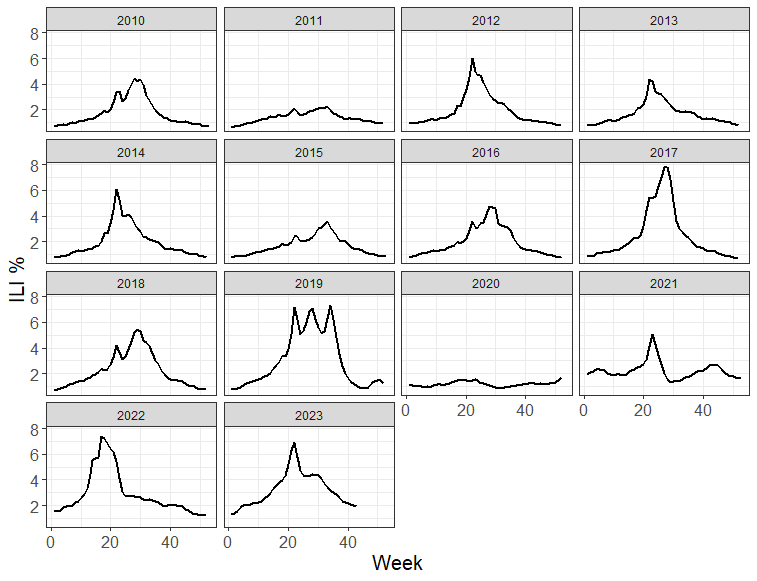
\includegraphics[scale=.7]{Images/us_ili_seasons.png}
    \caption{Percentage of outpatient visits with an influenza-like illness (ILI) in the US for seasons 2010 to 2023. Week 1 is the first week of August of the year the flu season begins and the last week of the season is the last week of July of the following year.}
    \label{fig:us_ili}
\end{figure}

Notable from the plots in figure \ref{fig:us_ili} is the regular trajectory of the ILI. With the exception of season 2020, the ILI begins low at week 1 and increases as the fall and winter progress until the ILI reaches a peak. As spring progresses to summer, the ILI decreases to low values. As \cite{osthus2019dynamic} point out, there is nearly always either a global or local peak at week 22 which typically corresponds to the week between Christmas and New Year's day. 
% The model formulated by \cite{osthus2019dynamic} was largely defined by the week 22 peak and influences the model we introduce in \ref{sec:model}. 
Whether local or global, the ILI holiday peak is generally expected and thought to be due to widespread holiday travel, school closure, or other unique social behavior   
\cite[]{ewing2017contact, garza2013effect}.
The only seasons when there was not a peak at week 22 were season 2022 where the season peak occurred particularly early and season 2020 which was greatly influenced by the COVID-19 pandemic.
% which would have affected patient visitations as well as reporting. 


Figure \ref{fig:ili_vs_week} shows ILI data from five states and the District of Columbia, locations which received particular attention in \cite{osthus2021multiscale}. The plots include the ILI data for all seasons from 2010 to 2023 in grey, and the black line is the per week ILI average over seasons. The patterns in the individual states are similar to the national level plots in figure \ref{fig:us_ili} in that the ILI rises in the fall and winter until it peaks and descends as the spring and summer progress. For these locations ILI regularly peaks, either locally or globally, at or near week 22. 

 \begin{figure}
    \centering
    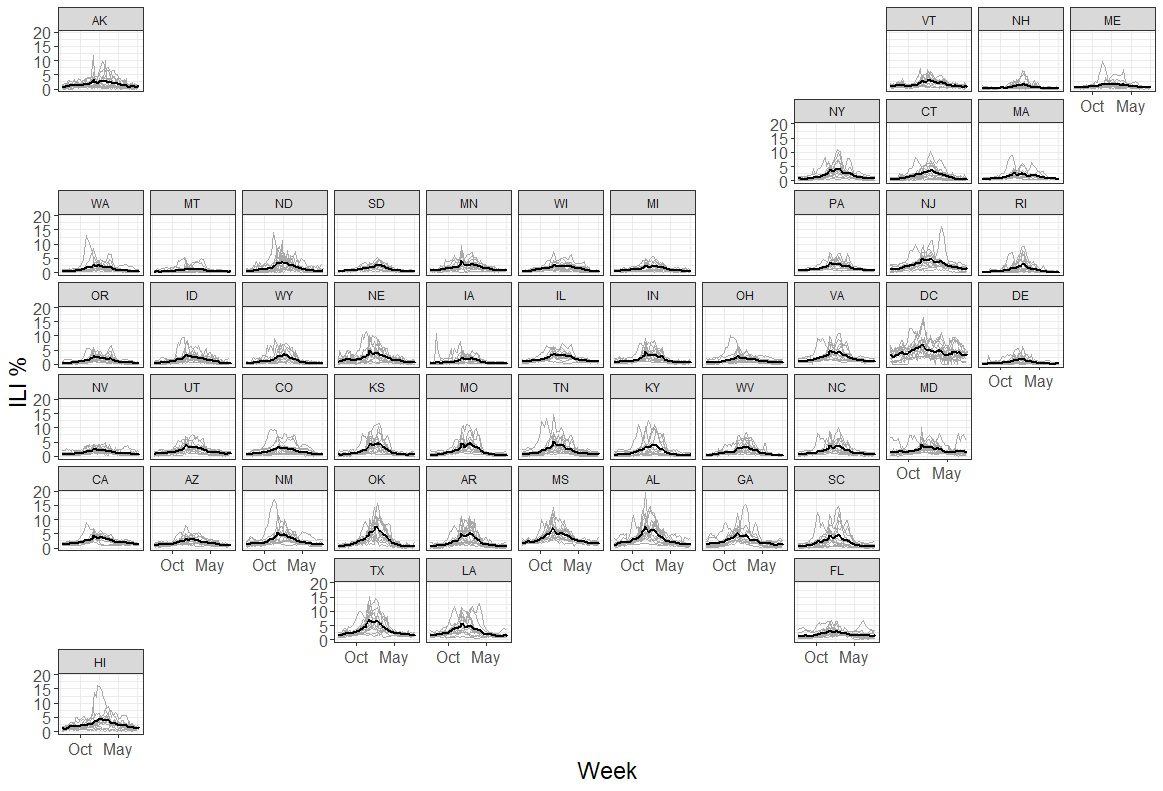
\includegraphics[scale=.7]{Images/ili_vs_week.png}
    \caption{Percentage of outpatient visits with an influenza-like illness (ILI) in five different states and the District of Columbia for seasons 2010 to 2023. Week 1 is the first week of August of the year the flu season begins and the last week of the season is the last week of July of the following year.
     Plots include lines for ILI\% from the 2010 flu season to 2023 (grey) and for the weekly ILI averaged over all seasons (black).}
    \label{fig:ili_vs_week}
\end{figure}





\subsection{Hospitalization Data}

Hospital admission data, used as the object of FluSight forecasting for the 2022 and 2023 seasons, is based on the CDC's National Healthcare Safety Network (NHSN) dataset entitled \textit{HealthData.gov COVID-19 Reported Patient Impact and Hospital Capacity by State Timeseries}. Several targets of respiratory illnesses including COVID-19, RSV, and influenza are reported weekly by most hospitals in the US. In February 2022 it became mandatory for all hospitals to report the number of COVID-19 and influenza hospitalizations, and since then reporting of hospitalizations has become widespread. These data were updated every Wednesday and Friday according to NHSN guidelines \cite[]{healthdata2024covidts}.

Figure \ref{fig:us_hosp} shows the weekly national hospitalizations for the 2022 and 2023 flu seasons. These plots show similarities to the ILI plots in \ref{fig:us_ili} in that at the early weeks of the season hospitalizations are low, but they increase in the fall to a peak after which they decrease until the flu outbreak ends. For both the 2022 and 2023 seasons, the hospitalizations peaked during the same week as ILI, and in 2023 that peak occurred during the holiday week 22. Figure \ref{fig:hosp_vs_week} shows the 2022 and 2023 weekly hospitalizations for the same states from \ref{fig:ili_vs_week}. Similar to the national data, the peak in 2022 came early compared to the peak of 2023.
% Comparisons similar to those of the national data may be made here. 
% \jarad{Did you forget to make comparisons?}


\begin{figure}
    \centering
    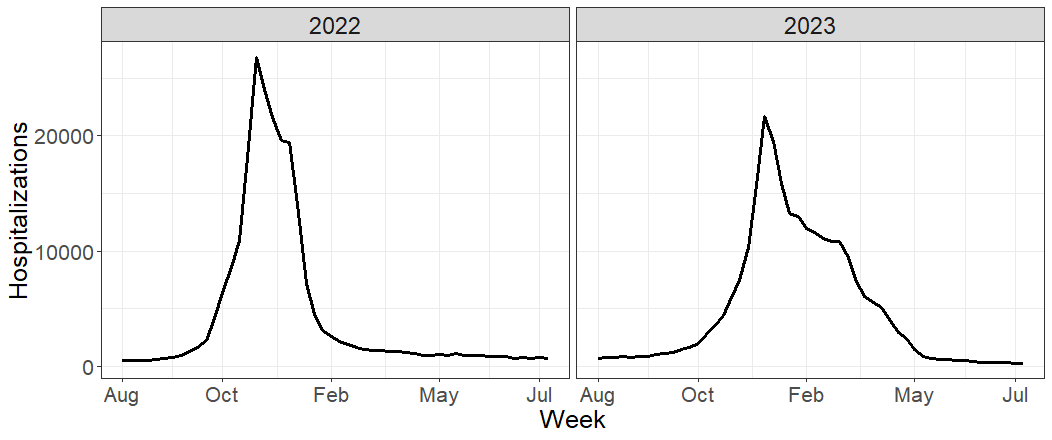
\includegraphics[scale=.5]{Images/us_hospitalizations.png}
    \caption{Weekly flu confirmed hospitalization counts at the national level for 2022 (left) and 2023 (right) flu seasons}
    \label{fig:us_hosp}
\end{figure}


\begin{figure}
    \centering
    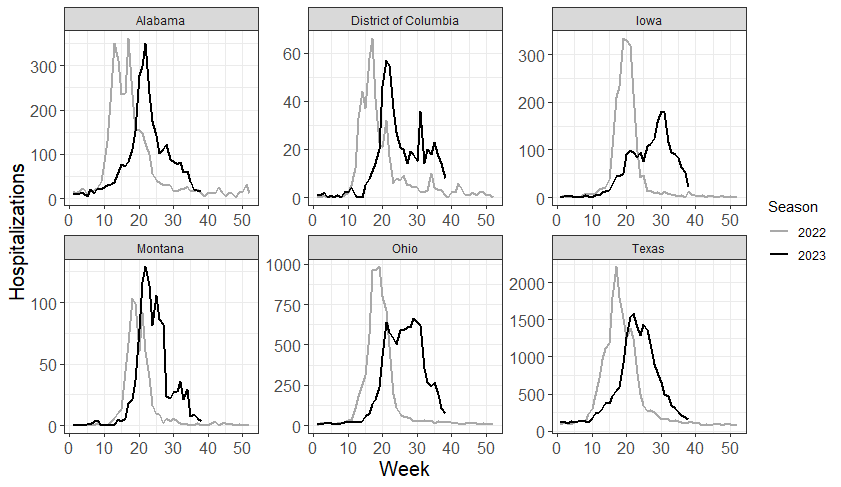
\includegraphics[scale=.65]{Images/hosp_vs_week.png}
    \caption{Weekly hospitalization counts for five states and DC for the 2022 (grey) and 2023 (black) flu seasons}
    \label{fig:hosp_vs_week}
\end{figure}


Comparing figures \ref{fig:ili_vs_week} and \ref{fig:hosp_vs_week} shows that ILI and hospitalizations share the similar pattern of increasing to a peak in the winter and decreasing thereafter. Figure \ref{fig:ili_vs_hosp} shows scatter plots with ILI\% on the $x$-axes and hospitalizations on the $y$-axes, revealing a positive somewhat linear relationship between the two variables. This relationship motivates the forecast models outlined in the next section. 

\begin{figure}
    \centering
    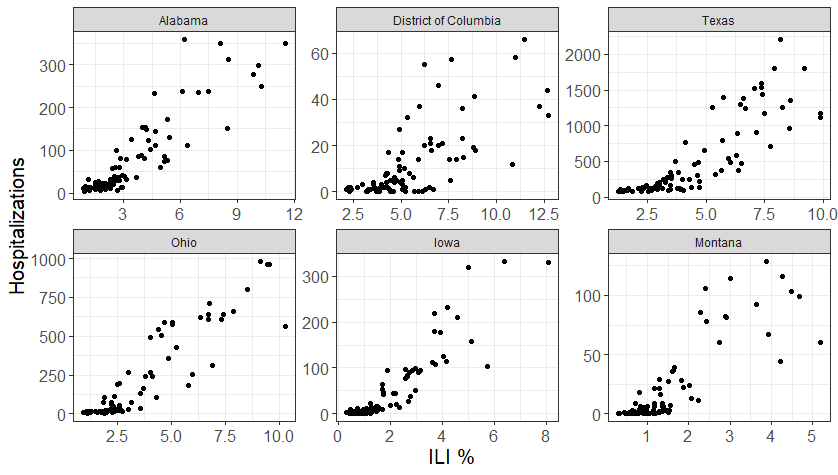
\includegraphics[scale=.6]{Images/ili_vs_hosp.png}
    \caption{Weekly flu confirmed hospitalization counts ($y$-axis) for five states and the District of Columbia for the 2022 and 2023 flu seasons plotted against ILI\% ($x$-axis)}
    \label{fig:ili_vs_hosp}
\end{figure}





% \subsection{Simple hospitalization model}
% \jarad{This should be the start of the methods section, so it should be a new section not subsection.}
% The CDC forecast competition between 2013 and 2020 seasons led to a number of advances and effective forecast models of ILI, and compared to weekly hospitalization data there is an abundance of ILI data. One contribution of this paper is that data and modeling techniques from forecasting ILI data may be used in forecasting hospitalizations. 
% A relationship between the ILI and hospitalization data exists, and to illustrate this we consider the model in equation (\ref{eq:simple_hosp_reg}). The model represents the hospitalizations for all weeks of one season and one state. For any state, $H_w$ is the hospitalization count at week $w$ and $ILI_w$ is the ILI value at the same week. The model is a squared polynomial regression with an autoregressive component of order 1. This is also known as an autoregressive with exogenous variables model (ARX(1)).
% \jarad{reference}

% \begin{equation}
%     H_{w} = \alpha_0 + \alpha_1 ILI_{w} + \alpha_2 ILI_{w}^2 + \phi H_{w-1} + \epsilon_{w}; \quad \epsilon_{w} \overset{iid}{\sim} N(0, \sigma_{\epsilon}^2)
%     \label{eq:simple_hosp_reg}
% \end{equation}
% \jarad{This model still doesn't make a lot of sense to me. I feel like we have talked about this before. Why isn't the H series centered around the ILI mean, e.g. 
% $\phi (H_{w-1} -\alpha_0 - \alpha_1 ILI_w + \alpha_2 ILI_w^2)$.}

% \begin{figure}
%     \centering
%     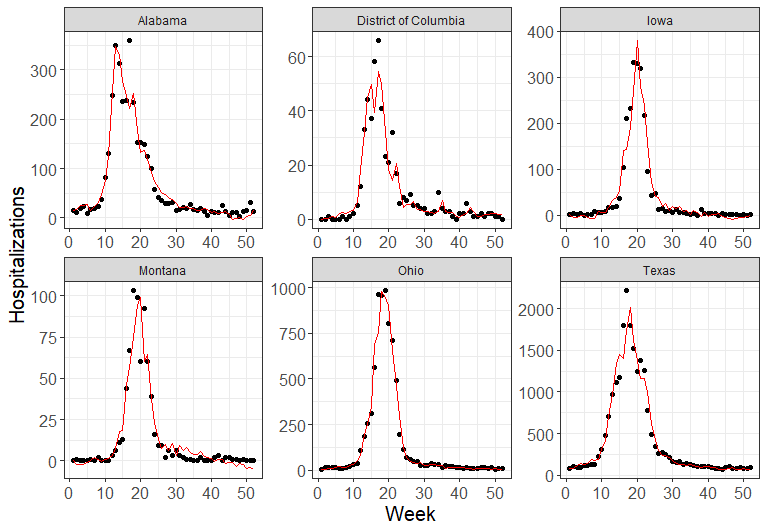
\includegraphics[scale=.8]{Images/hosp_preds_ili_22.png}
%     \caption{Weekly hospitalization counts during the 2022 flu season for 5 states and DC (black dots) and predicted weekly hospitalizations from the fit of model (\ref{eq:simple_hosp_reg}) (red lines)}
%     \label{fig:hosp_preds_ili_22}
% \end{figure}
% \jarad{Make the relationship between the data in the previous plot and this plot clear.}

% We fit this model for states individually under the 2022 flu season using the \texttt{lm} function in \texttt{R}.
% \jarad{It doesn't seem very important tha twe used lm in R.}
% Figure \ref{fig:hosp_preds_ili_22} shows the predicted hospitalizations from the fit model for several states. The black points are the true hospitalization counts and the red lines are the predicted hospitalizations from the fit model. 
% \jarad{Predicted or estimated?}
% The simple model does a decent job predicting hospitalizations, but forecasting future hospitalizations is more difficult. 
% \jarad{Why?}
% This, however, demonstrates that it is reasonable to model the behavior of hospitalizations as a linear function of ILI. 
% \jarad{You have a quadratic function of ILI not a linear function.}
% In the following two sections, nonlinear functions used in modeling and the proposed model are described.



\section{ILI and hospitalization forecast modeling} \label{sec:functions}

% \jarad{Why not start with the ILI model from Osthus et al? It makes a lot more sense to me to start with what has already been done and then expand upon what they have done. Later you have a section called ILI Model, but isn't this the ILI model?}

The typical behavior of the ILI data which starts at lower values in the late summer and fall but which increases to a peak, usually in December or January, followed by a decline motivates the use of a nonlinear function which follows of a similar trajectory for modeling ILI. Compartmental models are standard mathematical models used for disease outbreaks. One important compartmental model is the susceptible-infectious-recovered (SIR) model, which is used by some to model ILI data \cite[]{osthus2019dynamic, allen2017primer}. \cite{ulloa2019} chose to use the asymmetric Gaussian (ASG) function to model ILI data. The SIR and ASG models may both be appropriate to describe ILI behavior over the course of a flu season, however there may also be systematic behavior not captured by either, necessitating an additional model component to capture the discrepancy. In the first part of this section, we present an ILI model similar to the model in \cite{osthus2019dynamic}. With some generalization, the model may incorporate any appropriate nonlinear function, though the focus here is on the SIR and ASG functions which are defined. 

With the aim of forecasting hospitalizations, we also introduce a linear model of hospitalizations data with ILI as a predictive covariate. To forecast hospitalizations, ILI data is first forecasted and the forecast is then plugged in as a covariate in the hospitalization model, thus producing hospitalization forecasts. The hospitalization model is also defined in this section, and the section is concluded with descriptions of selected prior distributions, model implementation, and posterior sampling.
% In this section, we review the SIR and ASG functions as well as the lack of either model to capture certain behavior. We call the systematic deviation between the functional model and the observed behavior \textit{discrepancy}. 


\subsection{ILI Model} \label{sec:ili_model}

The proposed model for ILI for any location is given in (\ref{eq:ili_model}). Here $ILI_{s,w}$ is the ILI for flu season $s$ and week $w = 1, 2, ..., W$, where $W = 52$ or $W = 53$, depending on how many Sundays there are in a given season. The ILI is a proportion, so the Beta random variable is a natural selection for modeling. Under the parameterization in of the Beta distribution used in (\ref{eq:ili_model}) the expected value is $\pi_{s,w}$ and the variance is $\pi_{s,w}(1 - \pi_{s,w})/(1 + \kappa_s)$, making $\kappa_s$ a scale parameter. The nonlinear function $f_{\theta_s}(w)$ captures the trajectory of the ILI, and $\gamma_w$ is a discrepancy term for capturing the systematic patterns which $f_{\theta_s}(w)$ does not capture. 

\begin{equation}
    \label{eq:ili_model}
    \begin{flalign*}
        &ILI_{s,w} \overset{ind}{\sim} \text{Beta}(\pi_{s,w}\kappa_s,\; \kappa_s(1 - \pi_{s,w})) \\
        &\text{logit}(\pi_{s,w}) = f_{\theta_s}(w) + \gamma_w
    \end{flalign*}
\end{equation}
In \cite{osthus2019dynamic} $f_{\theta_s}(w) = \text{logit}(I_{s,w})$ where $I_{s,w}$ is the infectious compartment of the SIR model from (\ref{eq:sir_diff}) in section \ref{sec:sir_func}. In \cite{ulloa2019} $f_{\theta_s}(w) = ASG_{\theta}(w)$ from (\ref{eq:asg_function}) in section \ref{sec:asg_func}. In \cite{ulloa2019} modeling is done hierarchically over seasons. 
% The SIR and ASG functions are defined in the next two subsections.
% and $\gamma_w$ is modeled as a reverse random walk as in (\ref{eq:rw}). 


\subsection{Susceptible-Infectious-Recovered (SIR) compartmental model} \label{sec:sir_func}

The SIR compartmental model is a mathematical model used for modeling disease outbreaks and was introduced by \cite{kermack1927contribution}. Since then, compartmental models have become standard for modeling infectious diseases \cite[]{allen2008mathematical}, and many extensions have been made and studied \cite[for example]{simon2020sir, allen2017primer, van2008deterministic}. The SIR mathematical model includes three compartments and assumes that at any time $t>0$ every individual in a closed population belongs to exactly one compartment. The three compartments are susceptible ($S$), infectious ($I$), and recovered ($R$), and their interaction over the course of an outbreak is described by the differential equations in (\ref{eq:sir_diff}).    

\begin{equation}
    \label{eq:sir_diff}
    \frac{dS}{dt} = -\beta SI, \quad \frac{dI}{dt} = \beta S I - \delta I, \quad \frac{dR}{dt} = \delta I
\end{equation}
Here $S$, $I$, and $R$ represent the proportion of the population in each compartment such that $S + I + R = 1$ for all $t$. The trajectory is determined by the disease transmission rate $\beta > 0$ and the recovery rate $\delta > 0$. Respectively, these may be thought of as the expected proportion of susceptible individuals who will be infected by an infectious individual, and the expected rate of recovery to an immune state for a newly infected person. Whether or not a disease outbreak is classified as an epidemic is determined by the initial susceptible population $S_0$, or the susceptible population at time $0$, and the parameter $\rho = \delta/
\beta$. If $S_0/\rho > 1$, the outbreak is considered an epidemic. It is non-epidemic if $S_0/\rho \leq 1$ \cite[]{osthus2019dynamic}. Figure \ref{fig:sir_traj} shows the trajectory of the three compartments of an SIR model where the $S_0$ and $\rho$ were selected to match an outbreak that would classify as epidemic. In the case where $S_0 \leq \rho$, the trajectory for the $I$ compartment would never be increasing. The increase to a peak and subsequent decrease in the $I$ compartment of figure \ref{fig:sir_traj} suggest it is reasonable to model ILI by this compartment. Thus in modeling the ILI data, we consider the data to be analogous to the $I$ proportion of the population.

\begin{figure}
    \centering
    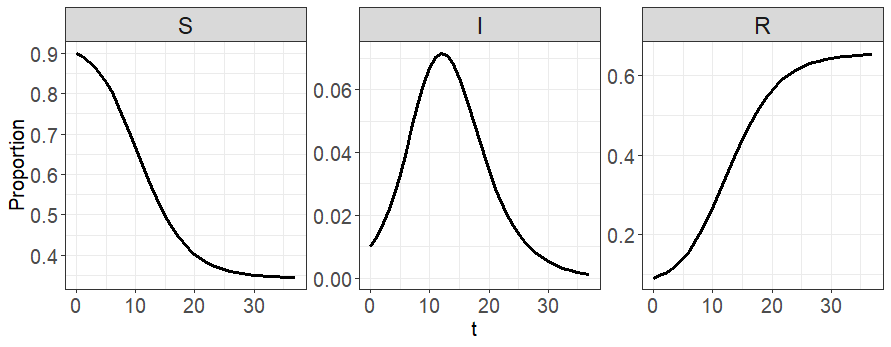
\includegraphics[scale=.6]{Images/sir_traj.png}
    \caption{Susceptible-infectious-recovered (SIR) model separated by compartments. The three compartments are the susceptible compartment (left), infectious (center), and recovered (right). In this example, $S_0/\rho > 1$.}
    \label{fig:sir_traj}
\end{figure}





\subsection{Asymmetric Gaussian (ASG) function} \label{sec:asg_func}
The ASG function is another example of a nonlinear function which can approximate the trajectory of the flu outbreak. The ASG was previously used by Ulloa to model and forecast ILI \cite[]{ulloa2019}, and it has been used to model vegetation growth and satellite sensor data \cite[]{lewis2020extracting, jonsson2002seasonality, hird2009noise, beck2006improved, atkinson2012inter}. The ASG is a modification of the asymmetric Gaussian distribution \cite[]{wallis2014two} and is characterized by its rise to a peak and fall from that peak which may not occur at the same rate, as shown in figure \ref{fig:asg_function}. The ASG function is denoted as $ASG_\theta(w)$ where $\theta = (\lambda, \nu, \mu, \sigma_1^2, \sigma_2^2)$, $\nu > 0$, $\lambda > 0$, $\mu \in (-\infty, \infty)$, $\sigma_1, \sigma_2 > 0$ and $w \in (1, ..., W)$ is week. The function is defined in (\ref{eq:asg_function}).

\begin{figure}
    \centering
    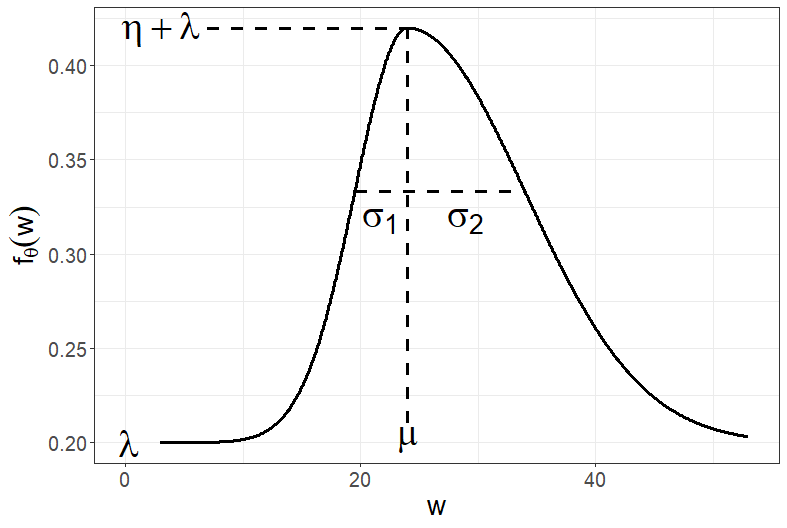
\includegraphics[scale=.45]{Images/asg_function.png}
    \caption{Example plot of asymmetric Gaussian (ASG) function showing the shape of the function in relation to the parameters $\lambda, \; \eta, \; \mu, \; \sigma_1, \; \text{and} \; \sigma_2$}
    \label{fig:asg_function}
\end{figure}

\begin{equation}
    \label{eq:asg_function}
    ASG_{\theta}(w) = 
    \begin{cases}
        \lambda + (\nu - \lambda) \text{exp}[-(w - \mu)^2/2\sigma^2_1], \;\;\; w < \mu \\
        \lambda + (\nu - \lambda) \text{exp}[-(w - \mu)^2/2\sigma^2_2], \;\;\; w \geq \mu
    \end{cases}
\end{equation}
For modeling in this manuscript, we use a slightly reparameterized version of the function in (\ref{eq:asg_function_rep}), where $\eta = \nu - \lambda > 0$. This constraint guarantees that the function has a peak greater than $\lambda$.

\begin{equation}
    \label{eq:asg_function_rep}
    ASG_{\theta}(w) = 
    \begin{cases}
        \lambda + \eta \text{exp}[-(w - \mu)^2/2\sigma^2_1], \;\;\; w < \mu \\
        \lambda + \eta \text{exp}[-(w - \mu)^2/2\sigma^2_2], \;\;\; w \geq \mu
    \end{cases}
\end{equation}



\subsection{Model discrepancy}


The SIR and ASG functions are useful for capturing the main trend of the ILI data, but as \cite{osthus2019dynamic} points out there may be systematic behavior that these or other possible functions may not capture. As noted in section \ref{sec:data}, figures \ref{fig:us_ili} and \ref{fig:ili_vs_week} show a regular peak at week 22 of the flu season. 
% It has been speculated that this drop may be the result of taking holiday from work or school or from the public wanting to avoid medical care around the holidays (??). 
Figures \ref{fig:asg_fits} and \ref{fig:discrepancy} are used together to illustrate the systematic discrepancy from a fitted function. Figure \ref{fig:asg_fits} shows the US ILI percentage for all flu seasons from 2010 to 2022 excluding 2020 with a best fit ASG function plotted over the ILI. The fits for each season were made by obtaining the maximum likelihood estimate (MLE) of a model given the ILI data where we assume the ASG function is the mean parameter of a Beta distributed random variable. Figure \ref{fig:discrepancy} shows the discrepancy between the model fit and the data for the same seasons. The grey lines show the difference between the data and the functions from figure \ref{fig:asg_fits} for each season, and the black line is the average by week over all seasons. The lines show that the ASG function typically underpredicts week 22 and overpredicts week 23. Perhaps for other weeks, like week 30 for example, there also tends to be systematic behavior not captured by the ASG function.


\begin{figure}
    \centering
    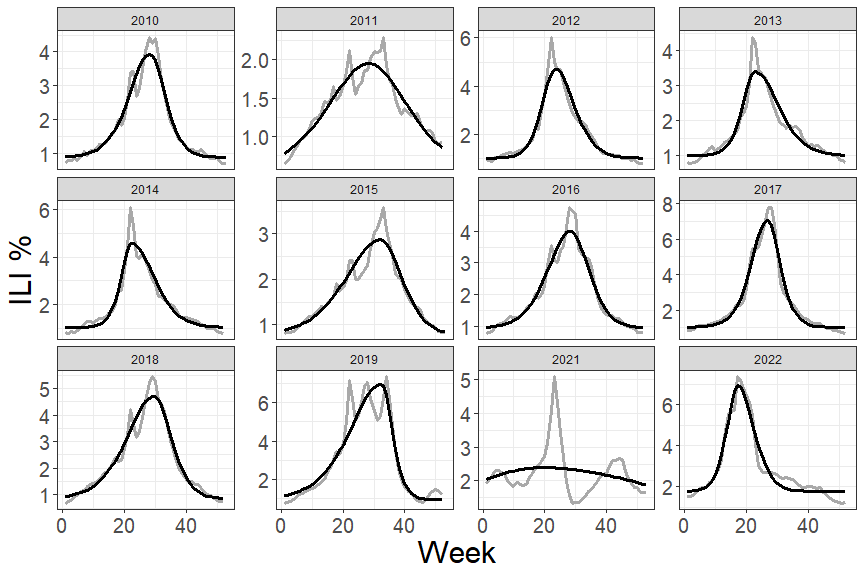
\includegraphics[scale=.5]{Images/asg_fits.png}
    \caption{Observed US national influenza-like illness (ILI) percentage for seasons 2010 to 2022 excluding 2020 (grey) overlaid with MLE of an asymmetric Gaussian (ASG) model for the ILI data (black)}
    \label{fig:asg_fits}
\end{figure}

\begin{figure}
    \centering
    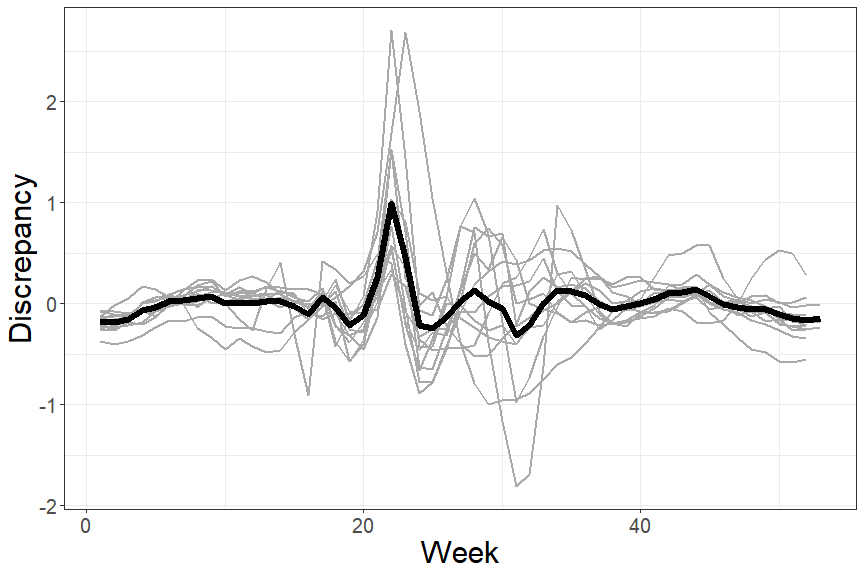
\includegraphics[scale=.45]{Images/discrepancy.png}
    \caption{Difference between observed US national influenza-like illness (ILI) and MLE fits for an asymmetric Gaussian (ASG) model for each season 2010 to 2022 excluding 2020 (grey) and the average difference of all seasons (black)}
    \label{fig:discrepancy}
\end{figure}


The term $\gamma_w$, where $w$ is the season week, is included in (\ref{eq:ili_model}) to capture the per week discrepancy between ILI and the function. Modeling discrepancy has been used in uncertainty analysis of simulators to capture systematic differences between mathematical models and 
reality \cite[]{ma2022multifidelity,brynjarsdottir2014learning,arendt2012improving,kennedy2001bayesian}. Modeling discrepancy can lead to overfitting, particularly in forecasting scenarios, and may also lead to identifiability issues. 
Thus, care must be taken in setting parameter constraints as well as in the selection of prior distributions \cite[]{osthus2019dynamic,brynjarsdottir2014learning}. 
Modeling of the discrepancy for ILI was done by \cite{osthus2019dynamic} during the 2015 and 2016 flu seasons where their model outperformed all others in the CDC flu forecasting challenge \cite[]{osthus2019dynamic}. As in Osthus's model, $\gamma_w$ is modeled as a reverse random walk, as shown in (\ref{eq:rw}). 
\begin{equation}
    \label{eq:rw}
        \gamma_w|\gamma_{w + 1} &\overset{ind}{\sim} N(\gamma_{t+1},\sigma^2_{\gamma}), \quad
        \gamma_{W} &\sim N(0,\sigma^2_{\gamma_W})
\end{equation}
The idea for using the reverse random walk is that there are several previous seasons of ILI data, and assuming the random walk captures systematic behavior, fitting it hierarchically over seasons can assist in predicting future behavior in the current season. 
Reverse random walks have also been used with success in election forecasting and other flu forecasting models \cite[]{osthus2021multiscale, osthus2019dynamic, linzer2013dynamic}. The sum to zero constraint $-\gamma_1 = \sum_{w=2}^W \gamma_w$ is imposed on (\ref{eq:rw}) to improve identifiability. 



\subsection{ILI forecasts}
Model (\ref{eq:ili_model}) is fit via Bayesian posterior updating. Future ILI forecasts are obtained via the posterior predictive distribution where for week $w$, the predictive distribution is obtained by integrating over the parameters $\pi_s$, $\kappa_s$, $\sigma^2_{\gamma}$, and $\sigma^2_{\gamma_W}$ as in (\ref{eq:ili_post}) where $p(\boldsymbol{\pi}_s, \kappa_s, \sigma^2_{\gamma}, \sigma^2_{\gamma_W} | \textbf{ILI})$ is the density function of the posterior distribution for the model parameters. If the current week is $w^*$ then the desired forecasts are for weeks $w^* + i$ where $i$ is a positive integer.

\begin{equation}
    \label{eq:ili_post}
    p(\widetilde{ILI}_{s,w^*} | \textbf{ILI}) = \int \int \int \int p(\widetilde{ILI}_{s,w^*} | \boldsymbol{\pi}_s, \kappa_s, \sigma^2_{\gamma}, \sigma^2_{\gamma_W}) p(\boldsymbol{\pi}_s, \kappa_s, \sigma^2_{\gamma}, \sigma^2_{\gamma_W} | \textbf{ILI}) d\boldsymbol{\pi}_s d \kappa_s d \sigma^2_{\gamma} d \sigma^2_{\gamma_W}
\end{equation}
% \jarad{It doesn't make sense to have 4 $\int$ here since $\pi_s$ is a vector.}
% \spencer{Isn't that captured in $d \pi_s$?}

% Below we consider four variations of model (\ref{eq:ili_model}). These include where $f_{\theta_s}(w) = ASG_{\theta}(w)$ and where $f_{\theta_s}(w) = \text{logit}(I_{s,w})$, $I_{s,w}$ being the infected compartment of an SIR model. For both function scenarios, models are fit where the discrepancy component $\gamma_w$ is included and excluded.



\subsection{Hospitalization model} \label{sec:hospital_model}

The second component for forecast modeling is the hospitalization model defined in (\ref{eq:final_hosp}). This is an example of an autoregressive model with exogenous variables where the autoregressive lag is one (ARX(1)) \cite[]{raftery2010online,ljung1987system}. Here $H_{s,w}$ is the number of hospitalizations for week $w$ in season $s$, $\epsilon_{s,w}$ is an error term distributed according to some distribution $D_s$ with mean parameter 0, scale parameter $\sigma_{\epsilon_s}$, and the additional parameter $\omega_s$ is the degrees of freedom parameter when $D_s$ belongs to the location-scale t (LST) family.  
% We further construct a forecast model for hospitalizations as a linear model of the ILI model. Similar to \ref{eq:simple_hosp_reg}, we select the model in (\ref{eq:final_hosp}). The desired outcome of this model is that the relationship between ILI and hospitalizations may be harnessed, and a future forecast of hospitalizations may be informed by a reasonable forecast for ILI as well as by past hospitalizations. 
\begin{equation}
    \begin{aligned}
    \label{eq:final_hosp}
    H_{s,w} &= \alpha_{0s} + \alpha_{1s} (ILI_{s,w} \times P) + \alpha_{2s} (ILI_{s,w} \times P)^2 + \phi H_{s,w-1} + \epsilon_{s,w}\\ 
    \epsilon_{s,w} &\overset{iid}{\sim} D_s(0, \sigma_{\epsilon_s}^2 \times P, \omega_s) %N(0, \sigma_{\epsilon}^2)
    \end{aligned}
\end{equation}
This model is for any location, and for fitting purposes $ILI_{s,w}$ is always multiplied by $P$ which is proportional to the population of the state or territory, in this case the total population divided by 50,000. This is done as a means of scaling so that the prior distribution assigned to  $\boldsymbol{\alpha}_s = (\alpha_{0s}, \alpha_{1s}, \alpha_{2s})$, $\sigma_{\epsilon_s}$, and $\omega_s$ might reasonably be the same for all states.

% Like the ILI model, model (\ref{eq:final_hosp}) was fit via MCMC sampling.
Like the ILI model, the hospitalization model in (\ref{eq:final_hosp}) is also fit via Bayesian posterior updating. To obtain forecasts for $H_{s, w^* + i}$, the ILI posterior predictive distribution is used along with the posterior distribution for the parameters in (\ref{eq:final_hosp}). We considered three scenarios for model (\ref{eq:final_hosp}). A model where $D_s$ belongs to the normal family (NORM), $D_s$ belongs to the LST family, and one where $H_{s,w}$ is replaced with $\text{log}(H_{s,w} + 1)$ and $D_s$ is from a normal family, or $H_{s,w} + 1$ is lognormally distributed (LNORM). The population value $P$ is excluded from the LNORM model, and we set $\boldsymbol{\alpha}_{22} = \boldsymbol{\alpha}_{23}$ to help with fitting. In the LNORM model, if the linear parameters are not set the same for seasons 22 and 23, the final variance was more prone to be extreme. Besides varying the distribution family of hospitalizations, we also considered $\alpha_{2s} = 0$ or there is no quadratic ILI term.



\subsection{Prior selection}


The priors selected for the ILI data model under both the SIR and ASG models largely follow the prior selections in \cite{osthus2019dynamic} and \cite{ulloa2019} with a few exceptions where changes improved numerical stability and/or we felt the adjusted prior made more sense for the problem. For model (\ref{eq:ili_model}), parameters which are common even when using different functions of $f_{\theta_s}(w)$ are $\kappa_s$, $\sigma_{\gamma}^2$, and $\sigma_{\gamma_W}^2$. For the SIR function $\theta_s = (S_{0s}, I_{0s}, R_{0s}, \alpha_s, \rho_s)$, and for the ASG function $\theta_s = (\alpha_s, \eta_s, \mu_s, \sigma_{1s}^2, \sigma_{2s}^2)$. For the hospitalization model in (\ref{eq:final_hosp}) the parameter to be estimated is $\Psi = (\alpha_{0s}, \alpha_{1s}, \alpha_{2s}, \phi, \sigma_{\epsilon_s}, \omega_s)$. 

% \begin{equation}
%     \label{eq:full_prior}
%     \begin{align*}
%     p(\theta, \Sigma, \kappa_s, \sigma_{\gamma}^2, \sigma_{\gamma_W}^2, \Psi) &= p(\theta)p(\Sigma)p(\kappa_s)p(\sigma_{\gamma}^2) p(\sigma_{\gamma_W}^2)p(\Psi), \\
%     p(\Psi) &= p(\alpha_{0s})p(\alpha_{1s})p(\alpha_{2s})p(\phi)p(\sigma_{\epsilon_s})p(\omega_s)
%     \end{align*}
% \end{equation}
% \jarad{What purpose is this serving?}

% Where the component parameters are shared for both SIR and ASG models, the individual parameter prior distribution assignments when $D_s$ from \ref{eq:final_hosp} is a normal distribution are in (\ref{eq:shared_priors}).
% \jarad{You cannot start a sentence like this. I think you intend for "where" to be a continuation of the equation, but the equation may be anywhere relative to the text, i.e. you cannot count on the "where" being immediately after the equation.}
The priors assigned were mostly noninformative, though in certain cases the prior distributions were selected for numerical stability as was the case for $\sigma_{\gamma}^2$ and $\sigma_{\gamma_W}^2$. For these two scale parameters only, rather than assigning a half-normal prior to the standard deviation parameters, as recommended by \cite{gelman2006prior}, the priors were assigned to the variance parameters. Univariate parameters were assigned either a normal distribution prior if the support is on $\mathbb{R}$, a half-normal prior if the support is nonnegative, or a truncated-normal prior to match a more specific support. Under the ASG model, $\theta_s$ is modeled hierarchically over seasons so that for each season the transformed parameter $T(\theta_s) \sim N(\theta, \Sigma$) and priors distributions are assigned to $\theta$ and $\Sigma$.



% Because parameter identifiability is lost when modeling with a discrepancy term \cite[]{brynjarsdottir2014learning}, additional constraints on the prior distributions should be made to improve identifiability. 
Additional prior constraints were made to improve parameter identifiability. In \cite{osthus2019dynamic} the initial value of the susceptible population compartment of the SIR model was set to $S_0 = 0.9$. The parameters $I_{0s}$, $\beta_s$, and $\rho_s$ were assigned informative priors. To improve identifiability when $f_{\theta_s}(w) = ASG_{\theta_s}(w)$ in (\ref{eq:ili_model}) we followed a modular Bayesian approach for fitting the parameters. A modular Bayesian approach involves multiple steps of parameter fitting where some parameters may be estimated without priors via maximum likelihood estimation or other means. Fitting the rest of the model parameters involves assigning priors and conditioning on the previously fit parameters. This has been done in computer modeling to improve identifiability and other issues, though \cite{liu2009modularization} warn this approach is not probabilistically sound if parameter inference is a priority \cite[]{jiang2015surrogate, arendt2012improving, liu2009modularization}. We carried out the modular fit by first estimating the maximum likelihood estimate (MLE) for the parameter $\lambda_s$ for each season in (\ref{eq:asg_function_rep}) and plugging in the MLE as a fixed value.


% \spencer{Blue stuff below will be either included further on or will be removed entirely

% \begin{equation}
%     \label{eq:shared_priors}
%     \begin{align*}
%         \kappa_s &\overset{ind}{\sim} N^+(0, 10,000^2) \\
%         \sigma_{\gamma}^2 &\sim N^+(0, .02^2) \\
%         \sigma_{\gamma_W}^2 &\sim N^+(\hat{\sigma}_W^2, 1^2) \\
%         \alpha_{0s} &\overset{ind}{\sim} N(0, 5^2) \\
%         \alpha_{1s} &\overset{ind}{\sim} N(0, 5^2) \\
%         \alpha_{2s} &\overset{ind}{\sim} N(0, 5^2) \\
%         \phi &\sim N(0, .4)\mathbbm{1}_{(-1,1)} \\
%         \sigma_{\epsilon_s} &\overset{ind}{\sim} N^+(0, 4^2) \\
%         \omega_s &\overset{ind}{\sim} N^+(0, 15^2)
%     \end{align*}
% \end{equation}
% \jarad{Generally introduce the distribution families in the methods, but the distributions themselves when performing the data analysis. Here I think you just need to say that you are using normals for unrestricted parameters, positive normals for positive parameters and a normal truncated on (-1,1) for the correlation. Also mention they are all independent (which I guess was done before.}

 

 



% }






% \section{Data Model} \label{sec:model}

% The modeling framework we introduce in this section is two-fold. To produce a forecast, we fit a model of only ILI data and fit a second model of hospitalization data with ILI as a linear covariate. The two models are fit separately, and a probabilistic forecast of ILI is then used as a predictive covariate for hospitalizations in a second model. We chose this type of framework because of the apparent relationship between ILI and hospitalizations, the availability of several flu seasons of ILI data compared to only two seasons of hospitalizations data, and the success of the ILI models introduced by \cite{osthus2019dynamic} and \cite{ulloa2019}. In this section we outline the two data models, the Bayesian analysis used for fitting including prior selection, and assess the posterior samples.


 
   











\subsection{Parameter estimation and posterior predictive sampling}
\label{sec:implementation_posterior}

The models were fit via Markov chain Monte Carlo (MCMC) sampling using the \texttt{cmdstanr} package which was developed and is maintained by the \cite{stan2024manual} \cite[]{gabry2022stan}. Stan implements Hamiltonian Monte Carlo (HMC) sampling with the No-U-turn sampler \cite[]{hoffman2014no}. The \texttt{cmdstanr} package provides several diagnostic statistics for assessing the sampler.
As mentioned, most model parameter prior distributions were intended to be uninformative. Appendix \ref{app:B_prior} shows plots of posterior distributions for select parameters from ILI and hospitalization models.

We assessed the model fit for four ILI models. These included the SIR and ASG models and models with and without discrepancy modeling. When discrepancy is included, the models are denoted as SIRD and ASGD. These models were fit using US national data from 2010 to 2023 flu seasons, where data from the 2020 season was excluded because of the unique behavior during that season. Assessment for hospitalization modeling was done for six different models. These include NORM, LNORM, and LST models, and models where a quadratic ILI term is included or excluded. To assess posterior sampling convergence, models were fit to data where ILI and hospitalization data up to week 14 of the 2023 season was included. Sampling was done with four chains where from each chain 60,000 posterior draws were sampled, and the first 10,000 draws were discarded as a burn-in. The $\hat{R}$ statistic \cite[]{vehtari2021rank} and the effective sample size ($ESS$) \cite[]{gelman2013bayesian} were calculated for each parameter. Tables \ref{tab:ili_diagnostics} and \ref{tab:hsop_diagnostics} summarize the maximum $\hat{R}$ and the minimum $ESS$ over all parameters for ILI and hospitalization models respectively. Forecast models for all other weeks of the season were fit using one chain of 60,000 draws where the first 10,000 draws were discarded as a burn-in. 
% \jarad{How long does this take to run? 8,000 inferential iterations seems very small.}
For parameters of the ASG models that were prone to cause trouble in posterior sampling, the starting values were set to be the MLEs. 

\begin{table}
\caption{Maximum $\hat{R}$ and minimum $ESS$ over all parameters for four ILI models fitted on US data for week 14 of the 2023 season}
\label{tab:ili_diagnostics}
\begin{center}
    \begin{tabular}{c|cccc}
     & ASG & ASGD & SIR & SIRD \\
     \hline
     $\hat{R}$ & $< 1.001$ & $< 1.001$ & $< 1.001$ & $1.001$ \\
     $ESS$ & 72,057 & 9,980 & 17,745 & 6,259 \\
    \end{tabular}
    \end{center}
\end{table}


\begin{table}
\caption{Maximum $\hat{R}$ and minimum $ESS$ over all parameters for six hospitalization models fitted on US data for week 14 of the 2023 season}
\label{tab:hsop_diagnostics}
\begin{center}
    \begin{tabular}{c|cccccc}
     & NORM & NORM^2 & LNORM & LNORM^2 &  LST &  LST^2 \\
     \hline
     $\hat{R}$ & $< 1.001$ & $< 1.001$ & $< 1.001$ & $< 1.001$ & $< 1.001$ & $< 1.001$\\
     $ESS$  & 71,266 & 73,554 & 46,747 & 54,975 & 7,660 & 62,663 \\
    \end{tabular}
    \end{center}
\end{table}



%  \begin{tabular}{ccccc}
% \hline
% \multicolumn{2}{c}{Set A} %%\\               %% <-- mistake
% %% \cline{1-2}                               %% <-- mistake
% &                                            %% <--  addition
% \multicolumn{2}{c}{Set B} \\\hline           %% <--  Changed
% Weight& Diameter    & Weight &Diameter      \\
% \hline
% \end{tabular}


To obtain forecast distributions of hospitalizations, draws from the posterior predictive distribution from the ILI model were used in conjunction with the posterior distribution of the hospitalizations model. When fitting model (\ref{eq:ili_post}), MCMC samples of $\widetilde{ILI}_{s,w:(w + 4)}$ were saved. Model (\ref{eq:final_hosp}) was fit and MCMC samples for the marginal distributions for the model parameters were saved. To obtain forecast distributions for $H_{s,w + i}$ where $i \in \{1,2,3,4\}$, the following steps are repeated $K$ times where $K$ is an integer for the number of desired samples. We set $K = 50,000$.

\begin{quote}
\begin{enumerate}[Step 1:]
  \item Sample $\widetilde{ILI}^*_{s,w:(w + 4)}$
  \item Sample $\alpha_{0s}^*$, $\alpha_{1s}^*$, $\alpha_{2s}^*$, $\phi^*$, $\sigma^*_{\epsilon_s}$, $\omega^*_s$ from respective marginal posterior distributions
  \item Sample $H^*_{s,w + i}$ from $D(\omega_s^*, \mu_{s, w + i}^*,\sigma^2_{\epsilon_s}$), where
  \begin{itemize}
    \item[] $\mu_{s,w + i}^* = \alpha_{0s}^* + \alpha_{1s}^* (ILI_{s,w + i}^* \times P) + \alpha_{2s}^* (ILI_{s,w + i}^* \times P)^2 + \phi^* H^*_{s,w + i - 1}$
  \end{itemize}
   \item Repeat step 3 for $i \in \{1,2,3,4\}$ to obtain $H^*_{s,(w + 1):(w + 4)}$
  \item Repeat steps 1-4 $K$ times
\end{enumerate}
\end{quote}
The sample $\{H^*_{s,w + i}\}^K$ was then used as the probabilistic forecast for hospitalizations at week $w + i$. For the forecast competition analysis in section \ref{sec:analysis}, all negative values of $\{H^*_{s,w + i}\}^K$ were set to 0 to reflect realistic values of hospitalizations and comply with the FluSight forecasting rules.



% \subsection{Posterior predictive forecast} \label{posterior_forecast}

% Probability forecasts for state hospitalizations are obtained via the posterior predictive 

% During the season, weekly hospitalization data was updated on Wednesdays, and forecast submissions were due that evening. ILI data was updated on Fridays leaving a lag of one week between the two sets of data when submissions were made. Because of this lag, for the most recent week $w^*$, $H_{s,w^*}$ is fit according to (\ref{eq:final_hosp}) but where $ILI_{s,w^*}$ is replaced by the posterior predictive distribution in (\ref{eq:ili_post}). For a given state, \textbf{ILI} is all observed ILI values the last value being $ILI_{s,w^*}$, and $\boldsymbol{\pi}_s = (\pi_{s,1}, ..., \pi_{s,w^*-1})$. Note that $w^*$ may also be replaced by any future $w + i$, $i \in (0, 1, ..., W)$.

% \begin{equation}
%     \label{eq:ili_post}
%     p(\widetilde{ILI}_{s,w^*} | \textbf{ILI}, 
%     \textbf{H}) = \int_{\Pi \times \mathcal{K}} p(\widetilde{ILI}_{s,w^*} | \boldsymbol{\pi}_s, \kappa_s) p(\boldsymbol{\pi}_s, \kappa_s | \textbf{ILI}, \textbf{H}) d(\boldsymbol{\pi}_s \times \kappa_s)
% \end{equation}



% Future hospitalization forecasts come from the posterior predictive distribution. We are interested in forecasting $\tilde{H}_{s,w + i}$ where $i \in (1, 2, 3, 4)$ meaning we forecast hospitalizations for 1, 2, 3, and 4-weeks ahead. The posterior predictive distribution of $\tilde{H}_{s,w + i}$ is defined in (\ref{eq:forecast_posterior}). Here $\Psi = (\beta_{0s}, \beta_{1s}, \beta_{2s}, \phi, \sigma_{\epsilon_s}, \nu_s)$ or the vector of all parameters in (\ref{eq:final_hosp}).
% %$\Psi = (\boldsymbol{\theta}, \boldsymbol{\beta})$


% \begin{equation}
%     \label{eq:forecast_posterior}
%     \begin{align*}
%         p(\tilde{H}_{s, w+i} |\textbf{H}, \textbf{ILI}) &= \\ \int_{\boldsymbol{\Psi} \times (0,1)} p&(\tilde{H}_{s, w+i} | \Psi) p(\Psi | \textbf{H}, \textbf{ILI}, \widetilde{ILI}_{s,w+i})  p(\widetilde{ILI}_{s,w+i} | \textbf{ILI})d (\Psi \times \widetilde{ILI}_{s,w+i}) 
%     \end{align*}
% \end{equation}

% After calculating (\ref{eq:forecast_posterior}) via MCMC sampling, the 23 quantiles requested by the CDC were calculated using the \texttt{quantile} function in \texttt{R} and truncated at 0. As stated, the focus of this paper is on forecasting hospitalizations when ILI is modeled according to the ASG function, but the work is heavily influenced by \cite{osthus2019dynamic}, so we compared forecasting ability to models where ILI is modeled similarly to the model proposed by Osthus.










% \begin{equation}
%     \label{eq:hosp_model}
%     \begin{flalign*}
%         \text{log}(H_w) = \alpha_0 + \alpha_1 \times \left[\text{logit}(I_{s,w})\right] + \epsilon_w; \quad \epsilon_w \overset{iid}{\sim} N(0, \sigma_{\epsilon}^2)
%     \end{flalign*}
% \end{equation}

% \begin{equation}
%     \label{eq:hosp_model}
%     \begin{flalign*}
%         \text{log}(H_w) = \alpha_0 + \alpha_1 \times \left[\text{log}(I_{s,w}) - \text{log}(1 - I_{s,w})\right] + \epsilon_w; \quad \epsilon_w \overset{iid}{\sim} N(0, \sigma_{\epsilon}^2)
%     \end{flalign*}
% \end{equation}

% \begin{equation}
% \label{eq:hosp_mod}
%     \begin{flalign*}
%         H_w &= \alpha_0_s + \alpha_1_s (I_{s,w} \times P) + \alpha_2_s (I_{s,w} \times P)^2 \\ &+ \alpha_3_s (I_{s,w} \times P)^3 + \phi_s H_{s, w-1} + \epsilon_{s,w} \\
%         \epsilon_{s,w} &\overset{iid}{\sim} N(0, \sigma^2_{\epsilon})  
%     \end{flalign*}
    
% \end{equation}

% \begin{equation}
% \label{eq:hosp_mod}
%     \begin{flalign*}
%         H_w &= \mu_s + \phi_s( H_{s, w-1} - \mu_s)+ \epsilon_{s,w} \\
%         \epsilon_{s,w} &\overset{iid}{\sim} N(0, \sigma^2_{\epsilon})  
%     \end{flalign*}
    
% \end{equation}

% where $\mu_s = \alpha_0_s + \alpha_1_s (I_{s,w} \times P) + \alpha_2_s (I_{s,w} \times P)^2 + \alpha_3_s (I_{s,w} \times P)^3$.

% Another option for modeling $H_w$ as a function of ILI is seen in 

% \begin{equation}
%     \label{eq:hosp_model_sqrt}
%     \begin{flalign*}
%         \sqrt{H_w} = \alpha_0 + \alpha_1 \times I_{s,w} + \epsilon_w; \quad \epsilon_w \overset{iid}{\sim} N(0, \sigma_{\epsilon}^2)
%     \end{flalign*}
% \end{equation}




\section{Simulation Study} \label{sec:simulation2}
In this section, we present a simulation study conducted for comparing ILI models and further assessing the hospitalization forecast model. US ILI data is used, and hospitalization data is simulated. 
A leave-one-season-out (LOSO) approach was combined with a Monte Carlo simulation approach. For each replication, we simulated log-hospitalizations for all weeks during seasons 2010, ..., 2022, excluding 2020, using the existing ILI data as a predictive covariate. Each season was in turn ``left-out" and treated as if it was the most recent season which we desired to forecast. Fitting and forecasting was then done for weeks 14, 20, 26, 32, and 38 of the left out season, giving two weeks that tend to occur as flu cases increase, two as cases decrease, and one that occurs when the cases may be increasing or decreasing. Week 20 is a week leading up to the holiday week 22 where ILI typically has a local peak. We were particularly interested in how important modeling discrepancy is for forecasting at week 20.

For the simulation of hospitalizations, the parameters $\boldsymbol{\alpha}_s = (\alpha_{0s}, \alpha_{1s}, \alpha_{2s})$ and $\sigma^2_{\epsilon_s}$ from the hospitalization model in (\ref{eq:final_hosp}) were considered the same across all seasons so that all $\boldsymbol{\alpha}_s = \boldsymbol{\alpha}$. 
The values for $\boldsymbol{\alpha}$, $\sigma^2_{\epsilon}$, and $\phi$ were estimated by fitting model (\ref{eq:final_hosp}) using ILI and hospitalization data from the 2022 season. For fitting, the hospitalization data was first log-transformed. We took $\boldsymbol{\alpha}_{\phi} = (\boldsymbol{\alpha}, \phi)$
and assigned the noninformative prior $p(\boldsymbol{\alpha}_{\phi}, \sigma^2_{\epsilon}) \propto 1/\sigma^2_{\epsilon}$. The marginal posterior distribution $\boldsymbol{\alpha}_{\phi} | \sigma^2_{\epsilon}, \boldsymbol{H_{22}}$ was then the established posterior multivariate normal distribution and $\sigma^2_{\epsilon} | \boldsymbol{H_{22}}$ the inverse-$\chi^2$ posterior distribution \cite[]{gelman2013bayesian}. The posterior means of those parameters were used as the values from which log-hospitalizations were simulated. The number of replicates in the simulation was 500.

% Predictive coverage was assessed at the 0.5 and 0.95 levels and measures what proportion of forecasts were captured by the corresponding intervals.
Model comparison was done by calculating the continuous ranked probability score (CRPS) and the logarithmic score (LogS) for each forecast. These scores are both proper scoring rules which evaluate the forecast distribution and density functions respectively. Proper scoring rules are the current standard for comparing performance between probabilistic forecasts and selecting the best forecasts according to the notion of maximizing sharpness subject to (auto-)calibration \cite[]{gneiting2007probabilistic, tsyplakov2013evaluation}. Proper scoring rules are commonly used in forecast comparison and have the property that a forecaster is incentivized to be honest in the reporting of their forecasts \cite[]{gneiting2007strictly, gneiting2014probabilistic}. The CRPS is defined in (\ref{eq:crps2}) and the LogS in (\ref{eq:logs2}). Here $F(\cdot)$ is the forecast distribution function, $f(\cdot)$ is the forecast density function, and $y^*$ is the observed targeted value of the forecast. The orientation of both scores is negative, meaning the smaller the score the better.

\begin{equation}
    \text{CRPS}(F, y^*) = \int_{-\infty}^{\infty} (F(x) - \mathbbm{1} (y^* \leq x))^2 dx
    \label{eq:crps2}
\end{equation}

% Having forecast distributions as posterior MCMC draws, the AE is calculated as the absolute difference between the sample median and the observed value.

\begin{equation}
    \text{LogS}(f, y^*) = -\text{log}(f(y^*))
    \label{eq:logs2}
\end{equation}
Both the CRPS and LogS are calculated using the \texttt{scoringRules} package in \texttt{R} \cite[]{jordan2019scoring}.
To calculate the LogS when given MCMC samples from a posterior predictive distribution, a continuous density function was first estimated via kernel density estimation. The CRPS is calculated using a quantile decomposition from \cite[]{laio2007verification}. 


% The number of replicates was selected by assessing the Monte Carlo coverage of absolute predictive error AE for 150 replicates. The AE mean and standard deviation were calculated across season, week, and horizon for each season, week and horizon included in the simulation. For each of these levels, we wanted a Monte Carlo confidence width to be less than 25, so we solved for $R$ the following 

% \[
%     25 = 2\times 1.96 * S_{m,s,w,h} / \sqrt{R}
% \]
% where $S_{m,s,w,h}$ is the SD for the MC AE for model $m$ at season $s$, week $w$, and horizon $h$. Across all $m, s, w, h$, the largest $R$ value was 1,030.533. 

% Tables \ref{tab:horizon_coverage} and \ref{tab:seasonweek_coverage} show the nominal coverage of forecasts for the simulated data. For each forecast, 50\% predictive interval was calculated with by finding the $25^{th}$ and $75^{th}$ percentiles and the 95\% predictive interval by the $2.5^{th}$ and $97.5^{th}$ percentiles. Table \ref{tab:horizon_coverage} show the coverage for each model averaged over all horizons as well as for horizons of 1-4 weeks ahead. Table \ref{tab:seasonweek_coverage} shows coverage averaged over the season weeks 14, 20, 26, 32, and 38 forecasts. None of the four models possess the nominal coverage as in each case the coverage is below the 0.5 or 0.95 targeted proportion. This is due more to the forecasts' inability to nominally cover the true ILI data and not the simulated hospitalization data. 




% \begin{table}
% \caption{}
% \label{tab:horizon_coverage}
% \begin{center}
%     \begin{tabular}{cccccc|ccccc}
%      &
%      \multicolumn{5}{c}{50\%}
%     & 
%     \multicolumn{5}{|c}{95\%} \\
%      Horizon week & Overall & 1 & 2 & 3 & 4 & Overall & 1 & 2 & 3 & 4\\ \hline
%      % Model & \\ \hline
%      ASG & \textbf{0.23} & 0.20 & 0.20 & \textbf{0.24} & \textbf{0.27} & 0.56 & 0.62 & \textbf{0.56} & 0.57 & \textbf{0.63} \\
%      SIR & 0.14 & 0.17 & 0.15 & 0.09 & 0.14 & 0.44 & 0.57 & 0.44 & 0.36 & 0.39\\
%      ASGD & 0.18 & 0.21 & 0.13 & 0.18 & 0.20 & 0.54 & 0.67 & 0.51 & 0.47 & 0.48\\ 
%      SIRD & 0.22 & \textbf{0.30} & \textbf{0.24} & 0.20 & 0.16 & \textbf{0.61} & \textbf{0.70} & 0.53 & \textbf{0.62} & 0.60\\ 
%     \end{tabular}
%     \end{center}
% \end{table}



% \begin{table}
% \caption{}
% \label{tab:seasonweek_coverage}
% \begin{center}
%     \begin{tabular}{cccccc|ccccc}
%      &
%      \multicolumn{5}{c}{50\%}
%     & 
%     \multicolumn{5}{|c}{95\%} \\
%      Season week & 14 & 20 & 26 & 32 & 38 & 14 & 20 & 26 & 32 & 38 \\ \hline
%      % Model & \\ \hline
%      ASG & \textbf{0.35} & 0.12 & 0.29 & 0.28 & \textbf{0.11} & 0.77 & 0.24 & 0.69 & \textbf{0.77} & \textbf{0.52} \\
%      SIR & 0.18 & 0.07 & 0.11 & 0.30 & 0.04 & 0.51 & 0.14 & 0.51 & 0.57 & 0.46\\
%      ASGD & 0.07 & 0.27 & \textbf{0.30} & 0.19 & 0.07 & 0.43 & 0.64 & \textbf{0.89} & 0.56 & 0.17\\ 
%      SIRD & 0.28 & \textbf{0.30} & 0.16 & \textbf{0.36} & 0.02 & \textbf{0.91} & \textbf{0.78} & 0.38 & 0.57 & 0.42\\ 
%     \end{tabular}
%     \end{center}
% \end{table}


Figures \ref{fig:overall_scores} - \ref{fig:logs_by_week_horizon} show boxplots of the CRPS and LogS for the four models. Figure \ref{fig:overall_scores} shows that the variation of overall CRPS is smallest for the ASG models and larger for the SIR models. The median scores for the SIR models also appears slightly higher than for the ASG models. 
When faceted by season in figure \ref{fig:crps_by_season}, the boxplots of the CRPS often show the same pattern for ASG and SIR models but not always. For example, the bulk of CRPS values for the SIRD model in 2019 appears to have smaller variation than the other models.
Figure \ref{fig:crps_by_week_horizon} shows CRPS boxplots faceted by week and horizon. Notable plots here are for week 20 where the two models accounting for the ILI discrepancy, ASGD and SIRD, have CRPS values with lower medians and lower variation than the two models not accounting for ILI discrepancy. This makes sense given the forecasts at week 20 are forecasting weeks, 22 and 23 where figure \ref{fig:discrepancy} shows a seasonal peak and trough. 


\begin{figure}
\centering
% \begin{subfigure}{.5\textwidth}
  \centering
  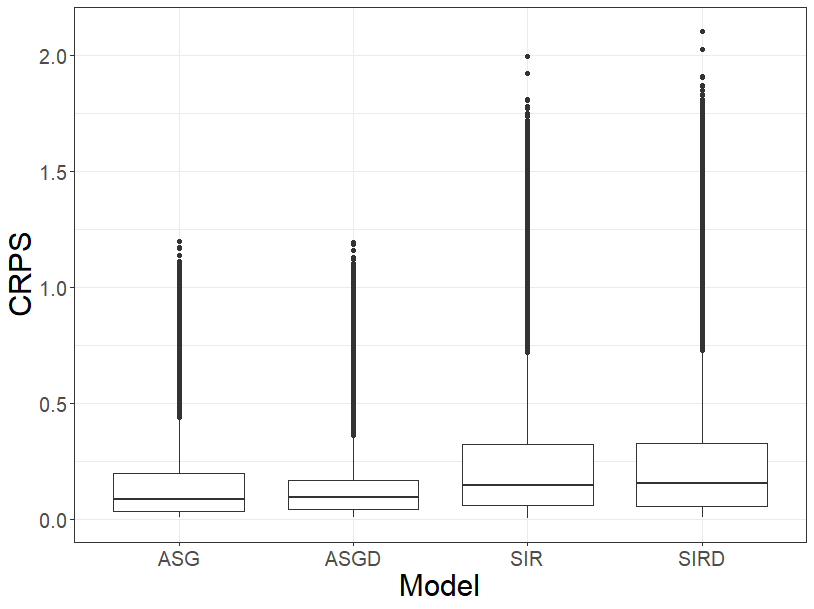
\includegraphics[scale=.35]{Images/overall_crps.png}
    % \caption{Boxplots of CRPS for the four ILI models over all seasons, weeks, and horizons in the simulation study}
% \end{subfigure}%
% \begin{subfigure}{.5\textwidth}
  \centering
  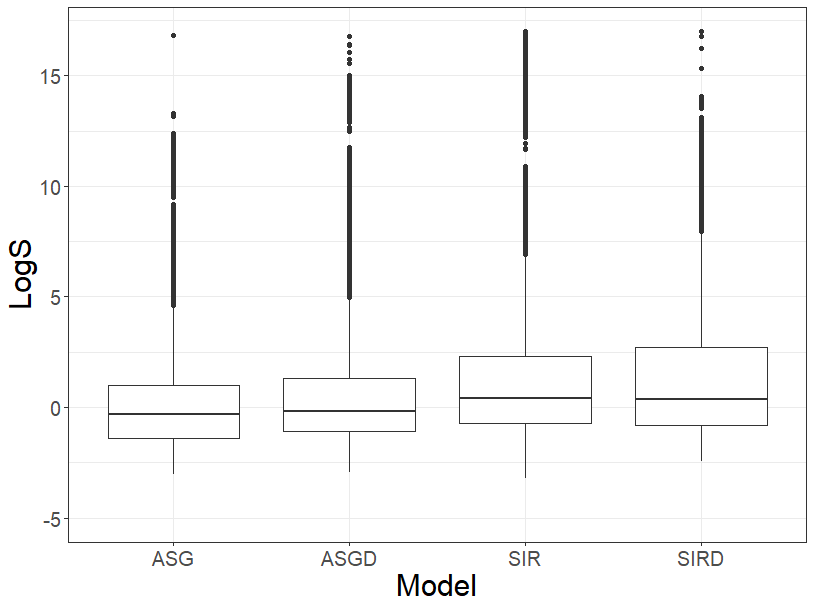
\includegraphics[scale=.35]{Images/overall_logs.png}
    % \caption{Boxplots of LogS for the four ILI models over all seasons, weeks, and horizons in the simulation study}}
% \end{subfigure}
\caption{Boxplots of the continuous ranked probability score (CRPS) (left) and logarithmic score (LogS) (right) for the four ILI models over all seasons, weeks, and horizons in the simulation study}
\label{fig:overall_scores}
\end{figure}

% \begin{figure}
%     \centering
%     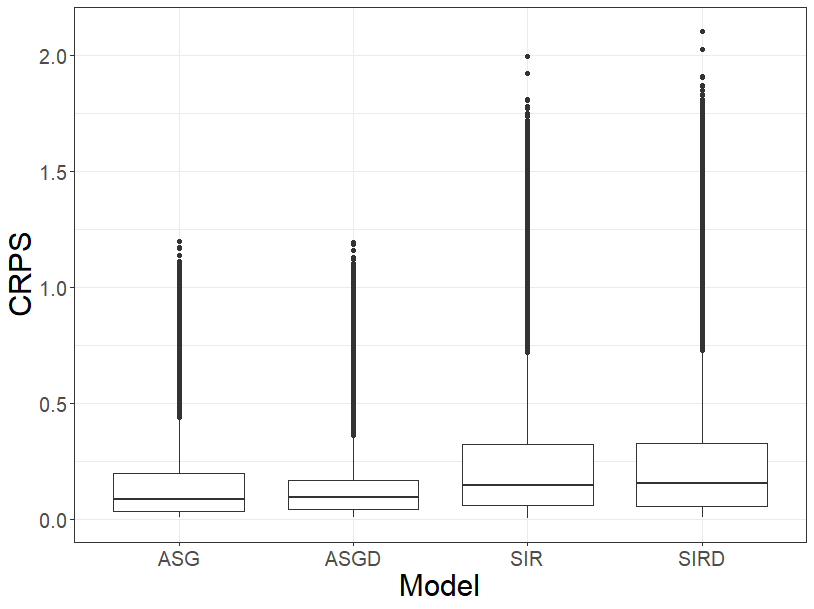
\includegraphics[scale=.6]{Images/overall_crps.png}
%     \caption{Boxplots of CRPS for the four ILI models over all seasons, weeks, and horizons in the simulation study}
%     \label{fig:crps_overall}
% \end{figure}


\begin{figure}
    \centering
    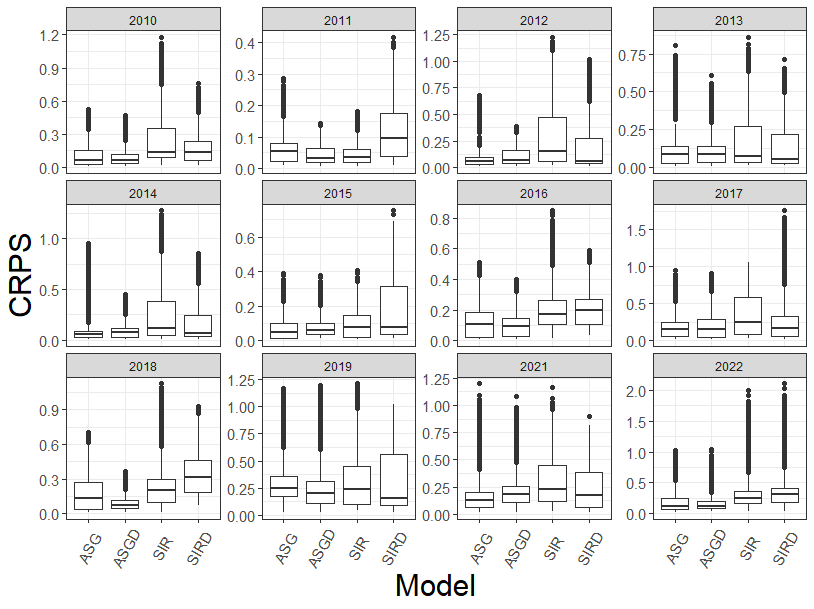
\includegraphics[scale=.5]{Images/crps_by_season.png}
    \caption{Boxplots of continuous ranked probability score (CRPS) for the four ILI models over all weeks and horizons in the simulation study faceted by season and including seasons 2010-2022, excluding 2020}
    \label{fig:crps_by_season}
\end{figure}

\begin{figure}
    \centering
    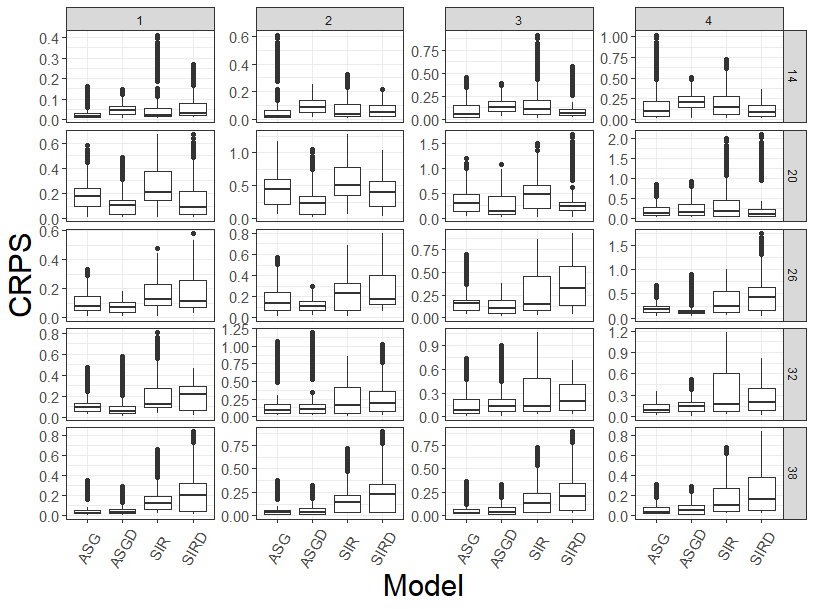
\includegraphics[scale=.5]{Images/crps_by_week_horizon.png}
    \caption{Boxplots of continuous ranked probability score (CRPS) for the four ILI models over all seasons in the simulation study faceted by horizon (x-axis) and week (y-axis). Horizons include 1-4 week ahead forecastss and weeks include weeks 14, 20, 26, 32, and 38 of the flu season}
    \label{fig:crps_by_week_horizon}
\end{figure}




% \begin{figure}
%     \centering
%     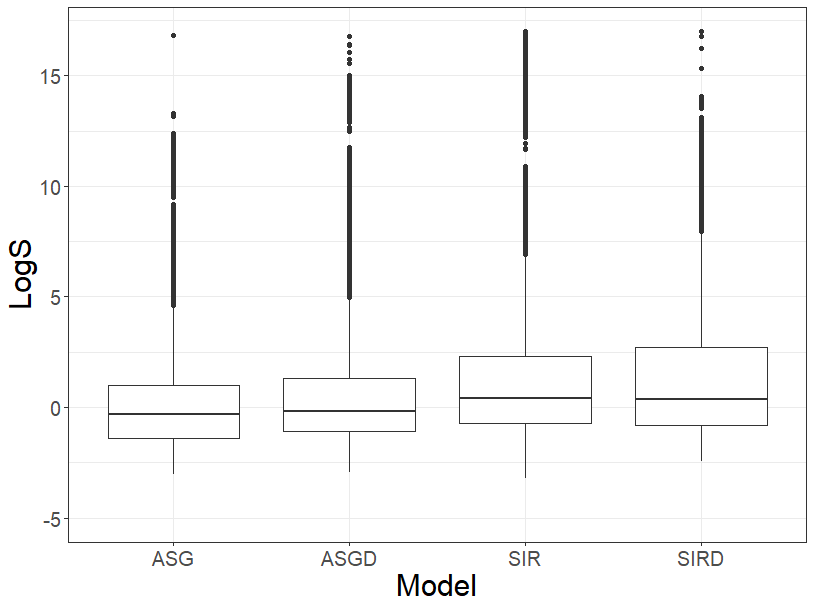
\includegraphics[scale=.6]{Images/overall_logs.png}
%     \caption{Boxplots of LogS for the four ILI models over all seasons, weeks, and horizons in the simulation study}}
%     \label{fig:logs_overall}
% \end{figure}


\begin{figure}
    \centering
    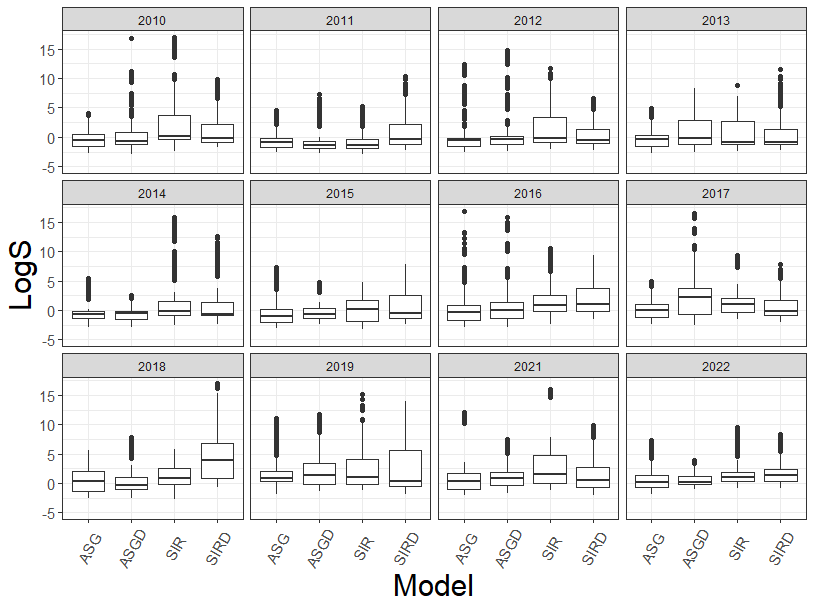
\includegraphics[scale=.5]{Images/logs_by_season.png}
    \caption{Boxplots of logarithmic score (LogS) for the four ILI models over all weeks and horizons in the simulation study faceted by season and including seasons 2010-2022, excluding 2020.}
    \label{fig:logs_by_season}
\end{figure}

\begin{figure}
    \centering
    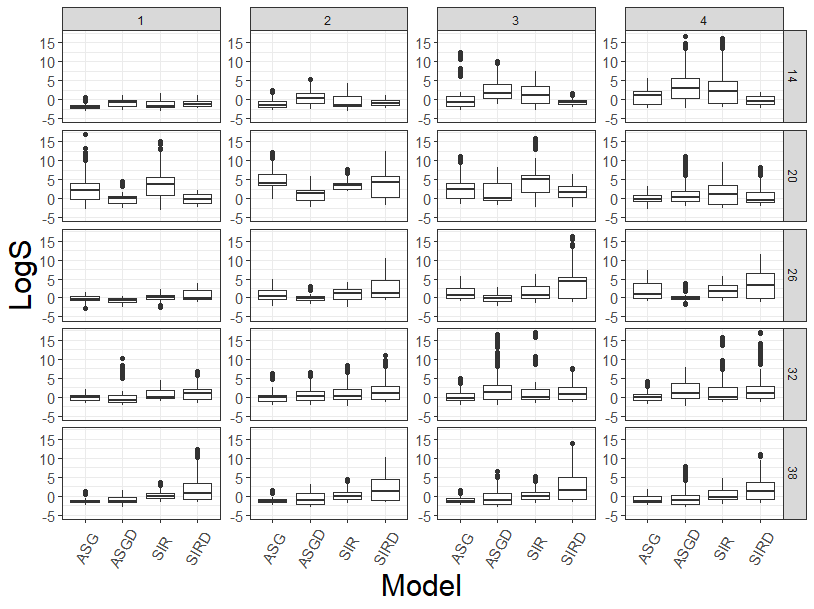
\includegraphics[scale=.5]{Images/logs_by_week_horizon.png}
    \caption{Boxplots of logarithmic (LogS) for the four ILI models over all seasons in the simulation study faceted by horizon (x-axis) and week (y-axis). Horizons include 1-4 week ahead forecasts and weeks include weeks 14, 20, 26, 32, and 38 of the flu season.}
    \label{fig:logs_by_week_horizon}
\end{figure}

% This simulation study shows that the predictive coverage of each of the four models considered is well below the nominal coverage based on constructing intervals using quantiles. 
Figures \ref{fig:logs_by_season} and \ref{fig:logs_by_week_horizon} show boxplots of the LogS for the simulated forecasts. Note that in these plots only values of less than 17 are included to improve visualization. 
% Figure \ref{fig:overall_scores} shows less dramatic differences in the LogS variation than the CRPS. There are a few notable differences between what the LogS captures vs. the CRPS.
The LogS plots show similar results to the CRPS, though there are some differences. For example, SIRD in figure \ref{fig:logs_by_season} tends to show smaller LogS variation relative to the other three models than is seen by the CRPS of SIRD in figure \ref{fig:crps_by_season}. 
We also note the smaller relative LogS variation than CRPS variation for SIRD when comparing figure \ref{fig:logs_by_week_horizon} with figure \ref{fig:crps_by_week_horizon}, particularly at week 14. 
Among the four models, ASG tends to have the lowest values in CRPS and LogS though this is not always the case. When forecasting weeks 21-23, the two models which model discrepancy in the ILI, ASGD and SIRD, tend to outperform the models not modeling the discrepancy. This confirms that there is value in modeling discrepancy at least during around the holiday weeks near week 22. 
% There are also slight differences in evaluation between the CRPS and the LogS. When scoring forecasts the two scores will not always recommend the same model(s). 
% Which of these or other scoring rules used in judging forecasts should reflect specific problem at hand.



\section{Analysis of forecasts for 2023 flu season}
\label{sec:analysis}

In this section we apply the forecast models to make forecasts of the 2023 flu season weekly hospitalizations. The scoring of the forecasts is in the context of the FluSight competition where each competing forecast was submitted as a set of 23 quantiles corresponding to the given probability levels $(0.010, 0.025, 0.050, 0.100, 0.150, …, 0.950, 0.975, 0.990)$. A single forecast is thus comprised of 11 predictive intervals and a median.
Forecasts of 1, 2, 3, and 4-week ahead hospitalization counts were requested, and forecasts were made at the state and national level. The first week of forecasting took place during the week of October 7, 2023, and the final week was the week of April 27, 2024 making 29 total weeks of forecasts.
 The same format was used during the 2021 and 2022 seasons and for the COVID-19 Forecast Hub \cite[]{mathis2024evaluation, bracher2021evaluating}. 
% Nearly teams participated and forecasts from over 40 models were submitted throughout the duration of the season. 
 Primary scores for evaluating each forecast were the weighted interval score (WIS), the log-weighted interval score (LWIS), and the relative weighted interval score (RWIS). The focus in this section will be on the LWIS (see appendix \ref{app:A_rwis} for RWIS based results).

The WIS is a proper scoring rule used for scoring quantile or interval forecasts \cite[]{gneiting2007strictly, gneiting2014probabilistic, bracher2021evaluating} and is defined in (\ref{eq:wis2}) where $Q$ is a forecast represented by all included quantiles, $B$ is the number of intervals,  $y^*$ is the observed value targeted by the forecast, $w_0 = 1/2$ and $w_b = \alpha_b / 2$ are weights for each interval, and $\alpha_b$ is the nominal level of the $b^{th}$ interval. $IS_{\alpha}$ is the interval score (IS), a proper scoring rule for a single interval as defined in (\ref{eq:is}). The goal of the forecaster is to minimize the WIS. The LWIS is the same as the WIS except that it is evaluated over the log of quantiles and the log of the observed value. 

\begin{equation}
\label{eq:wis2}
        WIS_{0,B}(Q, y^*) = \frac{1}{B + 1/2} \times (w_0\times |y^* - median| + \sum_{b=1}^B \{w_k \times IS_{\alpha_b}(Q, y^*) \} )
\end{equation}

\begin{equation}
\label{eq:is}
        IS_{\alpha}(l,r;y^*) = (r-l) + \frac{2}{\alpha}(l - y^*)\mathbbm{1}\{y^* < l\} + \frac{2}{\alpha}(y^* - r) \mathbbm{1}\{y^* > r\}
\end{equation}


We fit 24 forecast models for each location for all 29 weeks, and for each week forecast 1-4 week ahead hospitalizations. The 24 models included all combinations of ASG, ASGD, SIR, and SIRD ILI models, the NORM, LNORM, and LST hospitalization models, and both quadratic and linear hospitalization models. 
The prior distributions under the SIR model are in (\ref{eq:sir_prior}). Because we set $S_{0s} = 0.9$, prior distributions were assigned only to $I_{0s}$, $\beta_s$ and $\rho_s$, recalling the parameter for the recovery rate $\delta_s = \rho_s \beta_s$. Here $\mathbbm{1}_{A}$ represents the indicator function for values within the set $A$.

\begin{equation}
\begin{aligned}
    \label{eq:sir_prior}
        I_{0s} &\sim N(0.005, 0.03) \mathbbm{1}_{(0, .1)} \\
        \beta_s &\sim N^+(0.8, 0.3) \\
        \rho_s &\sim N^+(0.68, 0.08)
\end{aligned}
\end{equation}
For the ASG model, the MLE $\hat{\theta}_s = (\hat{\lambda}_s, \hat{\eta}_s, \hat{\mu}_s, \hat{\sigma}_{1s}^2, \hat{\sigma}_{2s}^2)$ was calculated and $\hat{\lambda}_s$ was accepted as a fixed value. The remaining estimates were used as starting values for posterior sampling. The transformation $T(\theta_s) = (\text{log}(\eta_s), \mu_s, \text{log}(\sigma_{1s}^2), \text{log}(\sigma_{2s}^2))$ was made, and a prior distribution was assigned to $T(\theta_s)$.
The prior distributions for the ILI model under the ASG function are shown in (\ref{eq:ili_prior}). These are slightly informative priors because for most parameters we have an idea what reasonable values may be. Here $m = (0.3, 23, 3.69, 4.7)$ and $C = \text{diag}(0.2, 5, 2, 2)$
where $\text{diag}(\cdot)$ 
is the diagonal matrix for the given entries.


\begin{equation}
\begin{aligned}
\label{eq:ili_prior}
                T(\theta_s) &\overset{ind}{\sim} MVN(\theta, \Sigma) \\
                T(\theta) &\overset{ind}{\sim} MVN(m, C)\\
                \Sigma &= \text{diag}(\zeta^2_1,...,\zeta^2_4) \\
                \zeta_i &\overset{ind}{\sim} N^+(0,4^2)
\end{aligned}
\end{equation}
Parameters shared by both the SIR and ASG models are the scale parameter $\kappa_s$ and the discrepancy parameters $\sigma_{\gamma}^2$ and $\sigma_{\gamma_W}^2$. These priors are in (\ref{eq:shared_ili_priors}). 

\begin{equation}
\begin{aligned}
    \label{eq:shared_ili_priors}
        \kappa_s &\overset{ind}{\sim} N^+(0, 10,000^2) \\
        \sigma_{\gamma}^2 &\sim N^+(0, .02^2) \\
        \sigma_{\gamma_W}^2 &\sim N^+(\hat{\sigma}_W^2, 1^2)
\end{aligned}
\end{equation}
Because of the limited information for estimating $\sigma_{\gamma_W}^2$, we selected an informative prior distribution by first estimating  $\hat{\sigma}_{\gamma_W}^2$. This was estimated for a given state by first calculating the MLE for $\theta_s$. 
% We set the likelihood function as $\mathcal{L}(\theta_s) = \prod_{w = 1}^W f_{\theta_s}(w)$ and  calculated $\hat{\theta}_s$ where $\label{eq:theta_hat}
%     \hat{\theta}_s = \underset{\theta_s}{\mathrm{argmin}} \, \mathcal{L}(\theta_s)$.
$\widehat{ILI}_{s,w}$ was then predicted such that $\text{logit}(\widehat{ILI}_{s,W}) = f_{\hat{\theta}_s}(W)$ for each season. Then $\hat{\sigma}_{\gamma_W}^2$ was calculated as the estimated variance over seasons of the differences $\text{logit}(\widehat{ILI}_{s,w}) - \text{logit}(ILI_{s,w})$. When $f_{\theta_s}(w)$ was the SIR function, $\widehat{\theta}_s$ was calculated using the \texttt{mle2} function in the \texttt{bblme} package \cite[]{bolker2023bblme} and the \texttt{ode} function in the \texttt{deSolve} package \cite[]{soetaert2010desolve} function in \texttt{R}. Where the ASG function was used,  $\hat{\theta}_s$ was calculated using the \texttt{optim} function.
The prior for the hospitalization models are in (\ref{eq:shared_hosp_priors}).

\begin{equation}
\begin{aligned}
\label{eq:shared_hosp_priors}
        \alpha_{0s} &\overset{ind}{\sim} N(0, 5^2)\\
        \alpha_{1s} &\overset{ind}{\sim} N(0, 5^2)\\
        \alpha_{2s} &\overset{ind}{\sim} N(0, 5^2) \\
        \phi &\sim N(0, .4)\mathbbm{1}_{(-1,1)} \\
        \sigma_{\epsilon_s} &\overset{ind}{\sim} N^+(0, 4^2) \\
        \omega_s &\overset{ind}{\sim} N^+(0, 15^2)
\end{aligned}
\end{equation}





\begin{figure}
\centering
\begin{subfigure}{.5\textwidth}
  \centering
  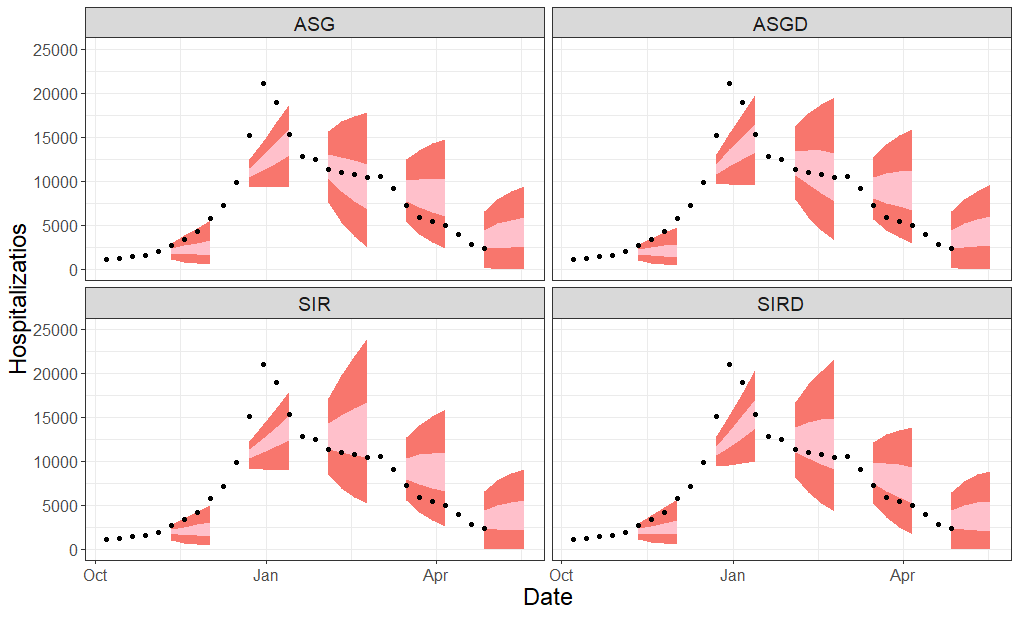
\includegraphics[width=1\linewidth,height=6cm]{Images/normal_forecasts_us.png}
  % \caption{A subfigure}
  % \label{fig:sub1}
\end{subfigure}%
\begin{subfigure}{.5\textwidth}
  \centering
  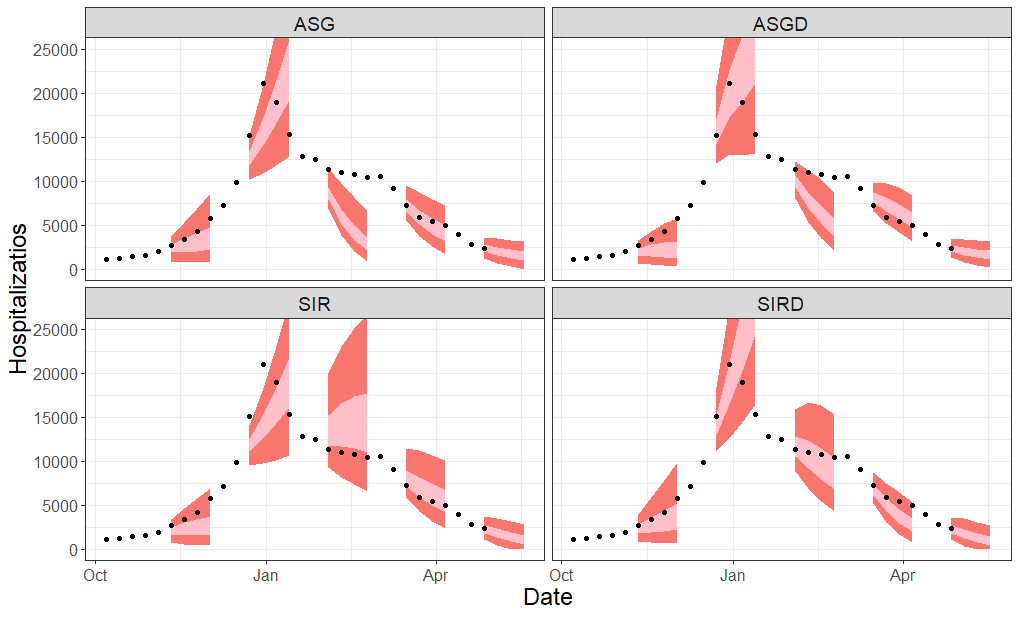
\includegraphics[width=1\linewidth, height=6cm]{Images/normal_sq_forecasts_us.png}
  % \caption{A subfigure}
  % \label{fig:sub2}
\end{subfigure}
\caption{Forecasts 1-4 weeks ahead for US hospitalizations during the 2023 season for weeks 14, 20, 26, and 32. Forecasts are separated by ILI model, and the hospitalization models are all normally distribution. The figure includes hospitalization forecasts where ILI is a linear predictor (left) and where ILI is a quadratic predictor (right). 50\% predictive intervals are pink and 95\% predictive intervals are red.}
\label{fig:normal_flu_forecasts}
\end{figure}

Figure \ref{fig:normal_flu_forecasts} shows 1-4-week ahead forecasts for US flu hospitalizations during the 2023 season under the NORM hospitalization model. The forecasts shown are for weeks 14, 20, 26, and 32. The predictive bands are the 50\% and 95\% predictive intervals.
These plots show a tendency to often underpredict hospitalizations. The quadratic models appear to do a better job predicting  hospitalizations at the season peak but a poorer job predicting after the peak, whereas the linear models seem to predict well or slightly overpredict after the peak. 
% From these figures, it's difficult to say whether ASG or SIR models predict better, but at least for the quadractic models the week 22 predictions are maybe slightly better than for the linear models.

Figure \ref{fig:us_lwis} shows model performance by LWIS for each week of the season for all 24 models of US hospitalizations. LWIS scores are grouped by ILI model, hospitalization model distribution, and by the linear or quadratic modeling. Here, a darker value represents a larger LWIS and worse forecast compared to lighter values. The weeks around the holiday week 22 are highlighted by a red band. In most cases, there appears to be a turning point in performance at or near week 22. The models which include discrepancy appear to forecast better around week 22, though they may not outperform the models without discrepancy through the whole season. 
Such is the case for the NORM and LST quadratic models and the linear LNORM models. It's also notable that for the SIR model, including discrepancy appears to make for poorer forecasts after week 22 whereas for ASG, including discrepancy appears to improve forecasts.



\begin{figure}
    
    % \centering
    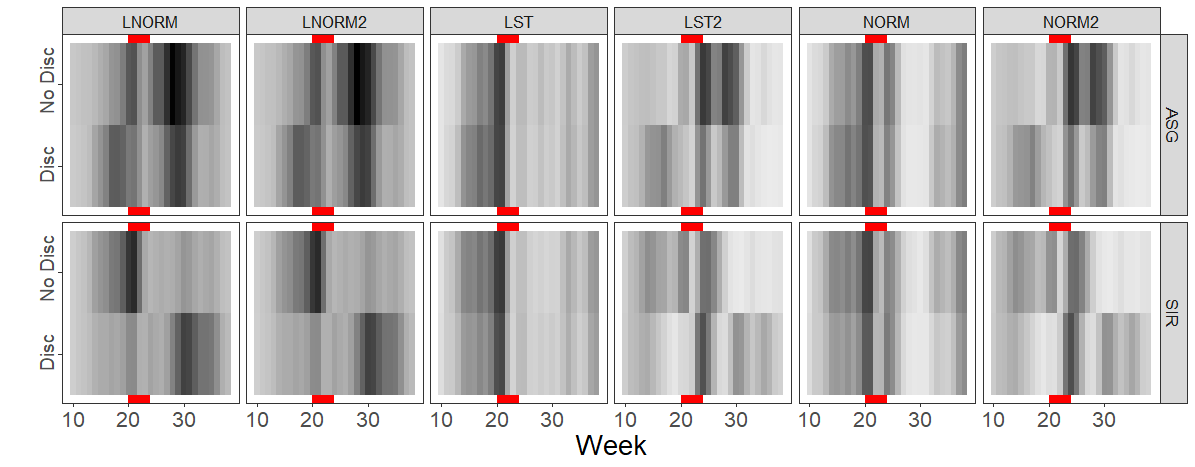
\includegraphics[scale = .5]{Images/lwis_us_full_season.png}
    \caption{Each plot shows the log weighted interval score (LWIS) for every week of the 2023 flu season with scores for models including discrepancy in the ILI model (top) and excluding discrepancy (bottom). Scores are separated by hospitalization distribution family and by ILI as a linear or quadratic predictor. Scores for models with an ASG ILI model are above while those with an SIR model are below. The lighter the shade, the lower the LWIS with low LWIS being better.}
    \label{fig:us_lwis}
\end{figure}

 

\begin{figure}
    
    \centering
    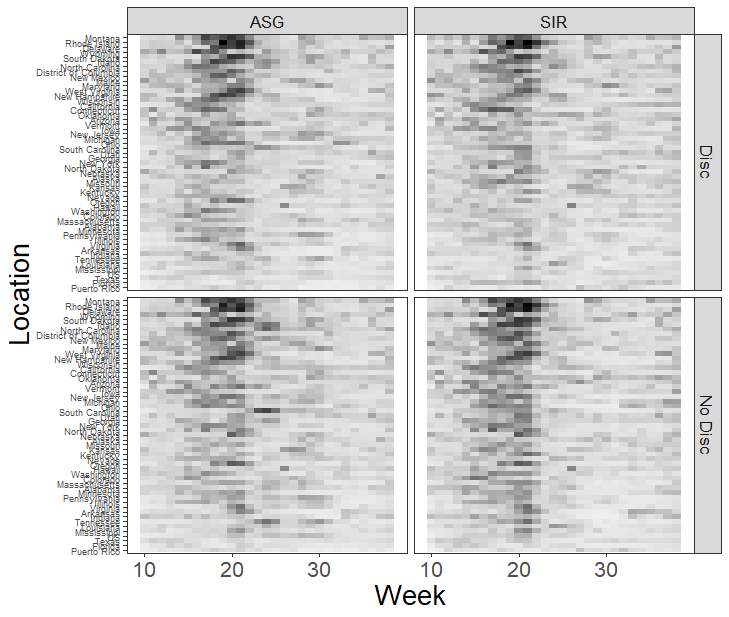
\includegraphics[scale = .7]{Images/lwis_by_traj_loc.png}
    \caption{Each plot shows the log weighted interval scores (LWIS) for all 50 US states, PR, DC, and national level forecasts at each week during the 2023 flu season. Scores are averaged over all horizons 1-4 weeks ahead. Scores are faceted by ILI model function (columns) and by whether or not discrepancy modeling was included (rows). The lighter the shade, the lower the LWIS with low LWIS being better.}
    \label{fig:lwis_by_traj_loc}
\end{figure}


\begin{figure}
    
    \centering
    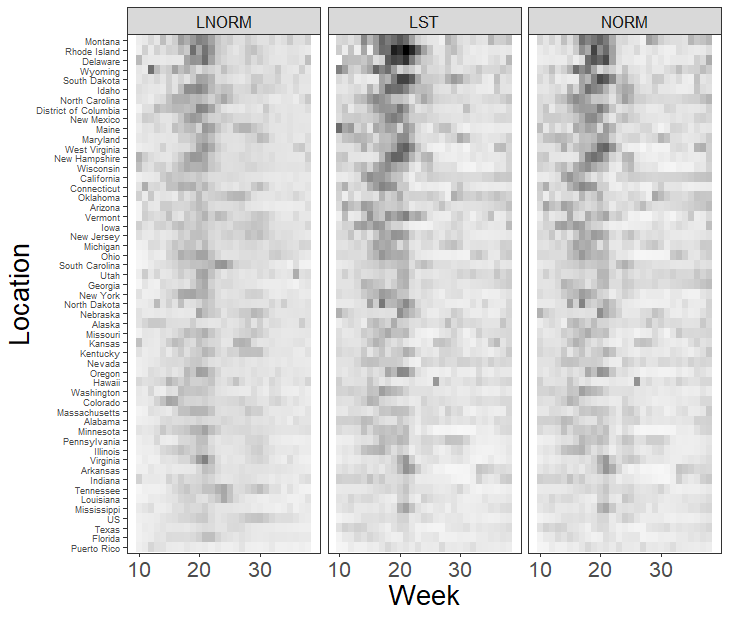
\includegraphics[scale = .7]{Images/lwis_by_dist_loc.png}
    \caption{Each plot shows the log weighted interval scores (LWIS) for all 50 US states, PR, DC, and national level forecasts at each week during the 2023 flu season. Scores are averaged over all horizons 1-4 weeks ahead. Scores are faceted by hospitalization model distribution. The lighter the shade, the lower the LWIS with low LWIS being better.}
    \label{fig:lwis_by_dist_loc}
\end{figure}

Figures \ref{fig:lwis_by_traj_loc} and \ref{fig:lwis_by_dist_loc} also show weekly forecast performance by LWIS, but all 53 locations are included. Overall, the weeks leading up to week 22 are the most difficult to forecast. In figure \ref{fig:lwis_by_traj_loc}, it appears that both the SIR and ASG models which include discrepancy perform slightly better than the models which do not. Figure \ref{fig:lwis_by_dist_loc} shows the LWIS across the whole season faceted by hospitalization model distribution. The LNORM model appears to perform the best during the weeks leading up to week 22. 
The season overall score, calculated as the mean LWIS over all locations and weeks, for all 24 models is shown in table \ref{tab:forecast_scores}. The first main takeaway is that the top four performing models are SIR ILI models with the LNORM hospitalization models. The next main takeaway is that overall the models which include discrepancy outperformed the models without discrepancy. 






\begin{table}
\caption{Overall scores for each of the 24 forecast models. The overall score is the log weighted interval score (LWIS) averaged over all locations, weeks, and horizons. The scores in the first two rows are for linear models, and the scores in the third and fourth rows are for quadratic models. The lowest WISs are bolded.}
\begin{tabular*}{\textwidth}
{@{\extracolsep{\fill}} 
    l 
    *{9}{c} 
    S[table-format=4.0]}
  & & \multicolumn{3}{c}{ASG} 
  & \multicolumn{3}{c}{SIR} \\ 
  \cmidrule{3-5} \cmidrule{6-8}
  & & LNORM & LST & NORM & LNORM & LST & NORM\\
  \midrule
  Linear & No Disc & 0.366 & 0.392 & 0.365 & \textbf{0.355} & 0.416 & 0.394 &\\ 
   & Disc & 0.358 & 0.391 & 0.365 & \textbf{0.343} & 0.382 & 0.354 &\\
  \midrule
  Quadratic & No Disc & 0.366 & 0.398 & 0.377 & \textbf{0.355} & 0.401 & 0.377 &\\ 
   & Disc & 0.358 & 0.390 & 0.369 & \textbf{0.343} & 0.378 & 0.356 &\\     
  \bottomrule
\end{tabular*}
\label{tab:forecast_scores}
\end{table}

It should not be assumed that these two takeaways will apply for future flu seasons. As suggested by the simulation study in the previous section, it may often be the case that the ASG ILI model is better for forecasting. Indeed, a close examination of figures \ref{fig:us_lwis}, \ref{fig:lwis_by_traj_loc}, and \ref{fig:lwis_by_dist_loc} shows that it is common for the ASG models to show better forecasting skill than the SIR models.



% Figure \ref{fig:us_lwis_box} shows boxplots of LWIS faceted by hospitalization model, separated by ILI model. The lognormal models tend to have higher LWIS scores than the LST and normal models. There doesn't appear to be a best model by LWIS, though it may be that overall discrepancy does improve forecasts made using the SIR function. Figure \ref{fig:state_lwis_box} is the same as figure \ref{fig:us_lwis_box} except that it shows plots for five states and DC. Interestingly the lognormal distribution for hospitalizations appears to outperform the LST and normal distributions. Again the discrepancy often appears to improve the forecasts and the SIR model. These boxplots also suggest that lognormal hospitalizations models and SIR models with discrepancy provide the best forecasts for Alabama, Montana, and Ohio.

% \begin{figure}
    
%     \centering
%     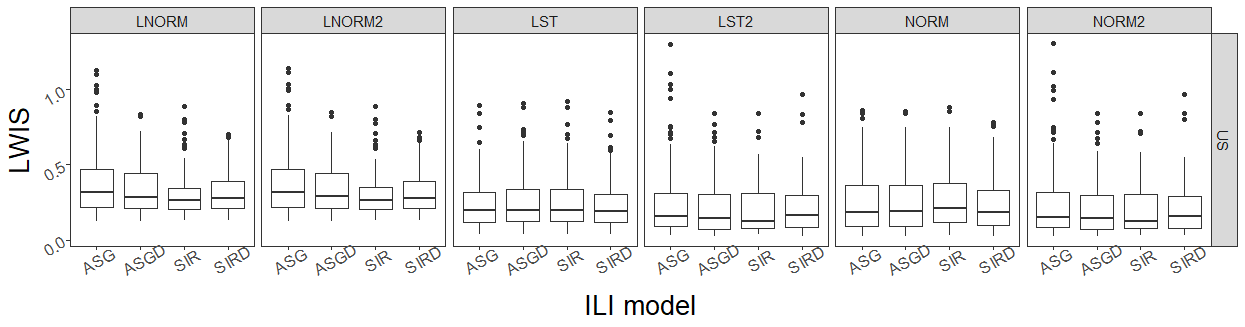
\includegraphics[width = 17cm, height = 5cm]{Images/us_lwis_box.png}
%     \caption{}
%     \label{fig:us_lwis_box}
% \end{figure}

% \begin{figure}
    
%     \centering
%     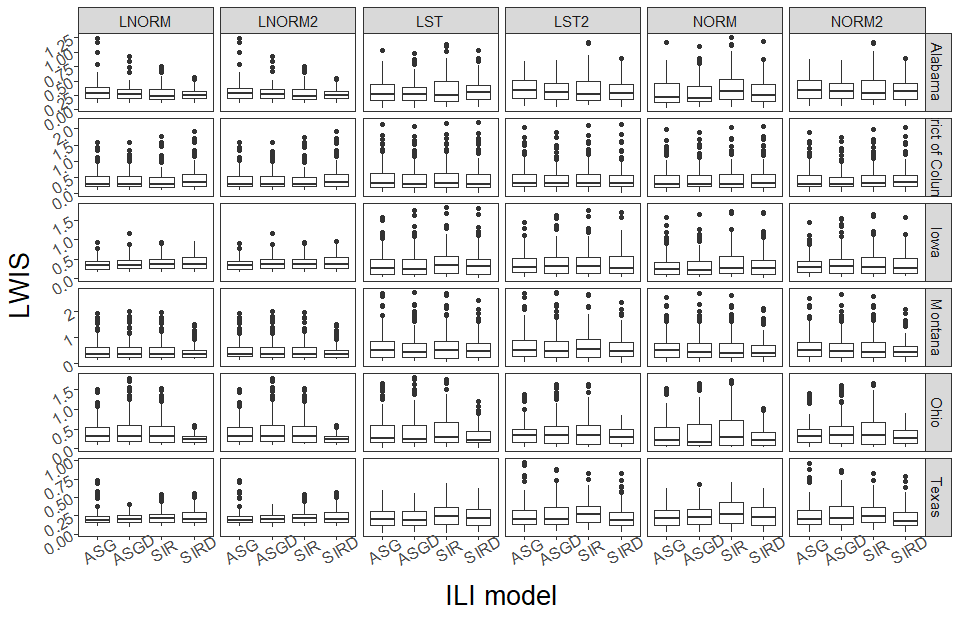
\includegraphics[scale = .6]{Images/state_lwis_box.png}
%     \caption{}
%     \label{fig:state_lwis_box}
% \end{figure}

% The lognormal and LST models at points during the season often displayed very wide and in some cases extreme predictive intervals. Interestingly the intervals for the LST models were not so wide when a square ILI term was included in the model, though it didn't necessarily lead to improved forecasts. This is seen in figure \ref{fig:t_sq_forecasts_us}.
% Figures \ref{fig:normal_sq_forecasts_us} and \ref{fig:log_sq_forecasts_us} also show forecasts for models excluding the square ILI term but for normal and lognormal distribution models. 





% \begin{figure}
%     \centering
%     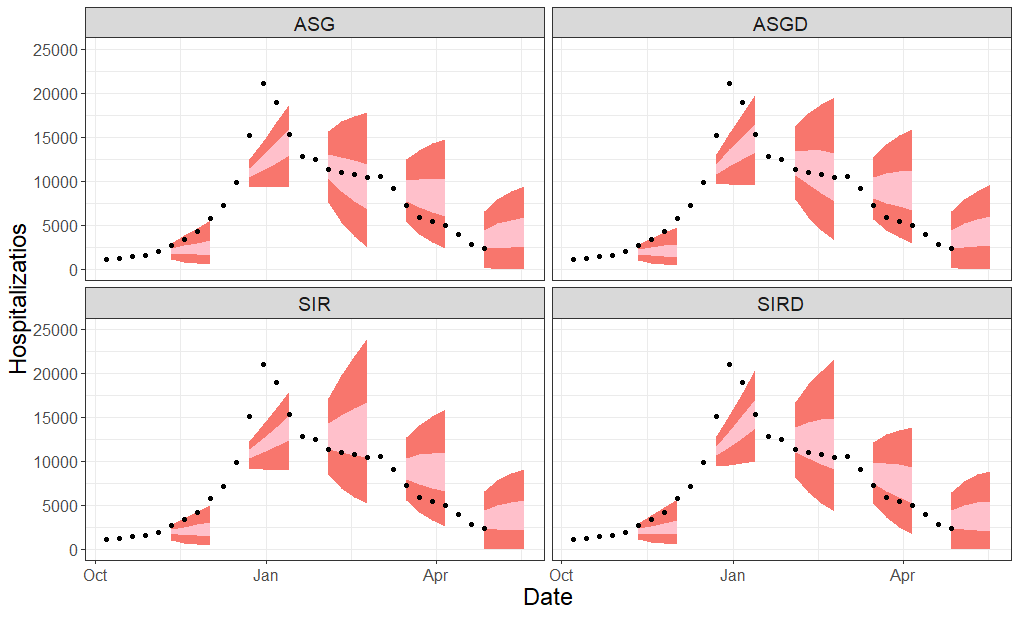
\includegraphics[scale=.5]{Images/normal_forecasts_us.png}
%     \caption{1-4 week ahead forecasts for US hospitalizations during the 2023 season for weeks 14, 20, 26, and 32. Forecasts are separated by ILI model, and the models are all normal and exclude the square ILI term. 50\% predictive intervals are pink and 95\% predictive intervals are red.}
%     \label{fig:normal_forecasts_us}
% \end{figure}

% \begin{figure}
%     \centering
%     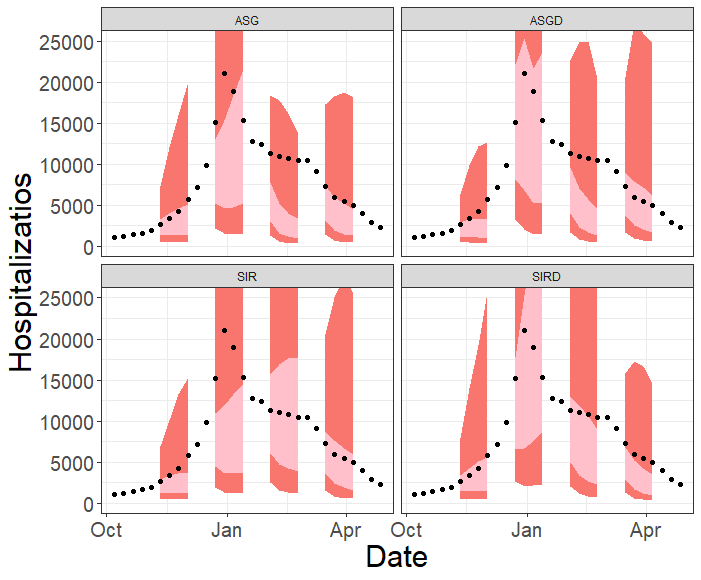
\includegraphics[scale=.5]{Images/log_forecasts_us.png}
%     \caption{1-4 week ahead forecasts for US hospitalizations during the 2023 season for weeks 14, 20, 26, and 32. Forecasts are separated by ILI model, and the models are all lognormal and exclude the square ILI term. 50\% predictive intervals are pink and 95\% predictive intervals are red.}
%     \label{fig:log_forecasts_us}
% \end{figure}

% \begin{figure}
%     \centering
%     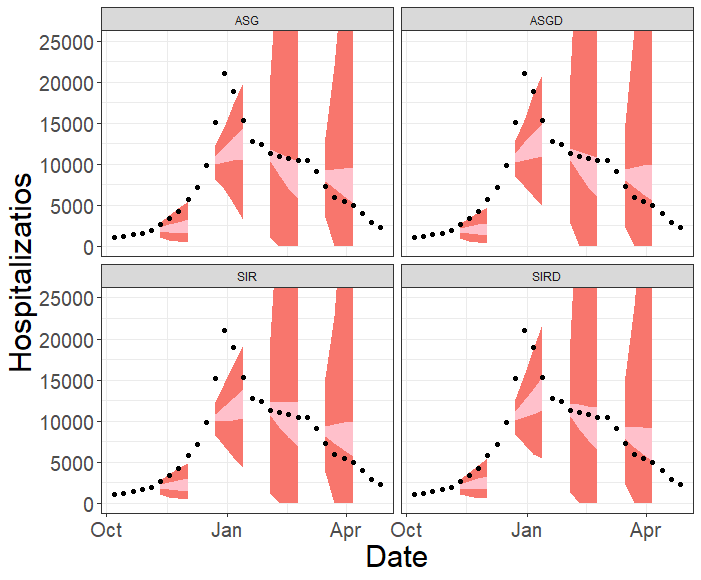
\includegraphics[scale=.5]{Images/t_forecasts_us.png}
%     \caption{1-4 week ahead forecasts for US hospitalizations during the 2023 season for weeks 14, 20, 26, and 32. Forecasts are separated by ILI model, and the models are all LST and exclude the square ILI term. 50\% predictive intervals are pink and 95\% predictive intervals are red.}
%     \label{fig:t_forecasts_us}
% \end{figure}










% \begin{figure}
%     \centering
%     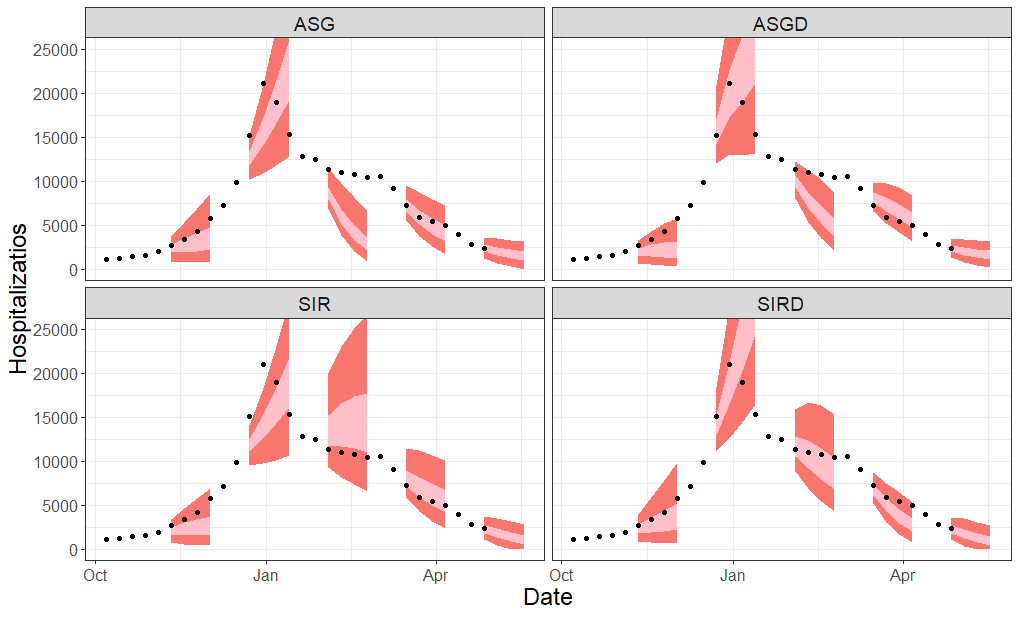
\includegraphics[scale=.5]{Images/normal_sq_forecasts_us.png}
%     \caption{1-4 week ahead forecasts for US hospitalizations during the 2023 season for weeks 14, 20, 26, and 32. Forecasts are separated by ILI model, and the models are all normal and include the square ILI term. 50\% predictive intervals are pink and 95\% predictive intervals are red.}
%     \label{fig:normal_sq_forecasts_us}
% \end{figure}

% \begin{figure}
%     \centering
%     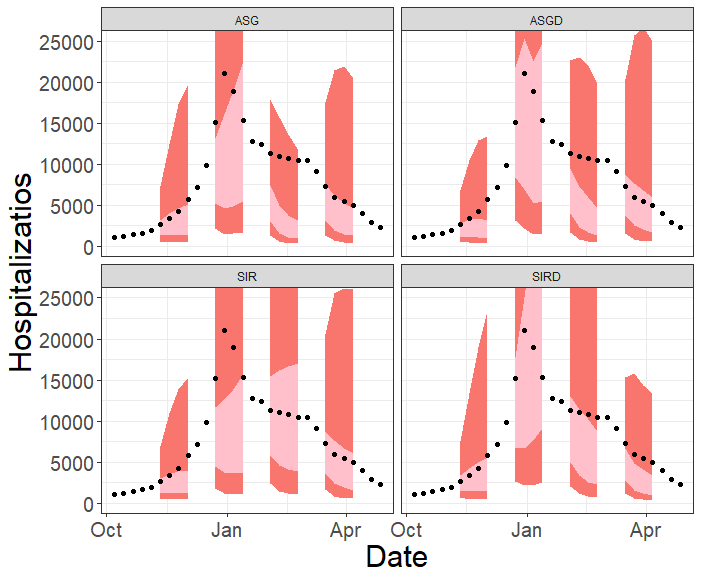
\includegraphics[scale=.5]{Images/log_sq_forecasts_us.png}
%     \caption{1-4 week ahead forecasts for US hospitalizations during the 2023 season for weeks 14, 20, 26, and 32. Forecasts are separated by ILI model, and the models are all lognormal and include the square ILI term. 50\% predictive intervals are pink and 95\% predictive intervals are red.}
%     \label{fig:log_sq_forecasts_us}
% \end{figure}

% \begin{figure}
%     \centering
%     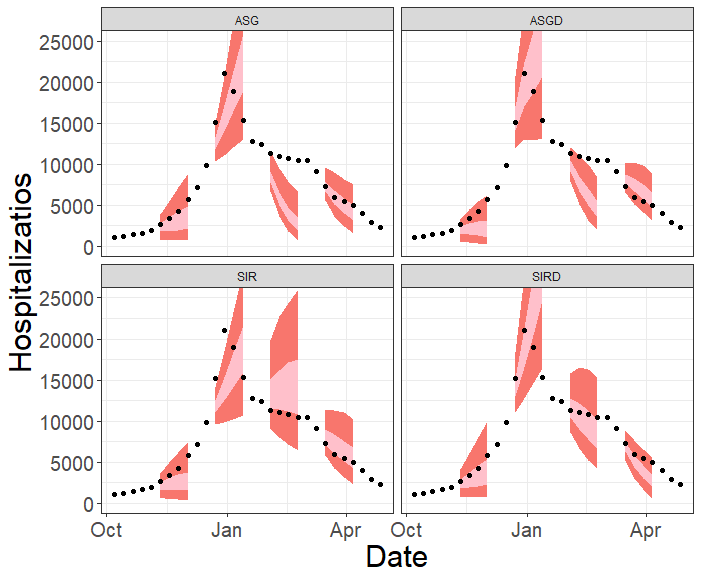
\includegraphics[scale=.5]{Images/t_sq_forecasts_us.png}
%     \caption{1-4 week ahead forecasts for US hospitalizations during the 2023 season for weeks 14, 20, 26, and 32. Forecasts are separated by ILI model, and the models are all LST and include the square ILI term. 50\% predictive intervals are pink and 95\% predictive intervals are red.}
%     \label{fig:t_sq_forecasts_us}
% \end{figure}









% \begin{figure}
%     \centering
%     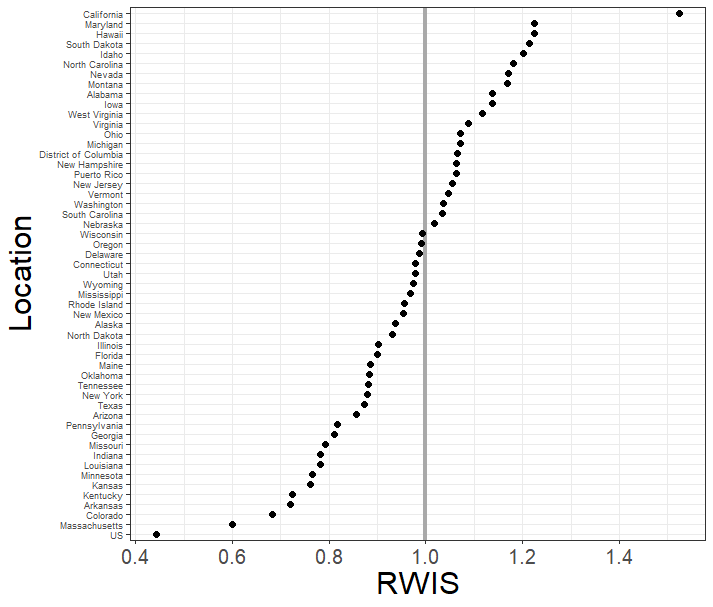
\includegraphics[scale=.5]{Images/asg_hosp_sq_ar1_rwis.png}
%     \caption{Overall median RWIS by location (black points) for forecasts made by a model including the ASG model without discrepancy, the normal hospitalization model with the square ILI term. The grey line at RWIS = 1 represents the RWIS for the baseline forecast.}
%     \label{fig:asg_sq_ar1_rwis}
% \end{figure}

% \begin{figure}
%     \centering
%     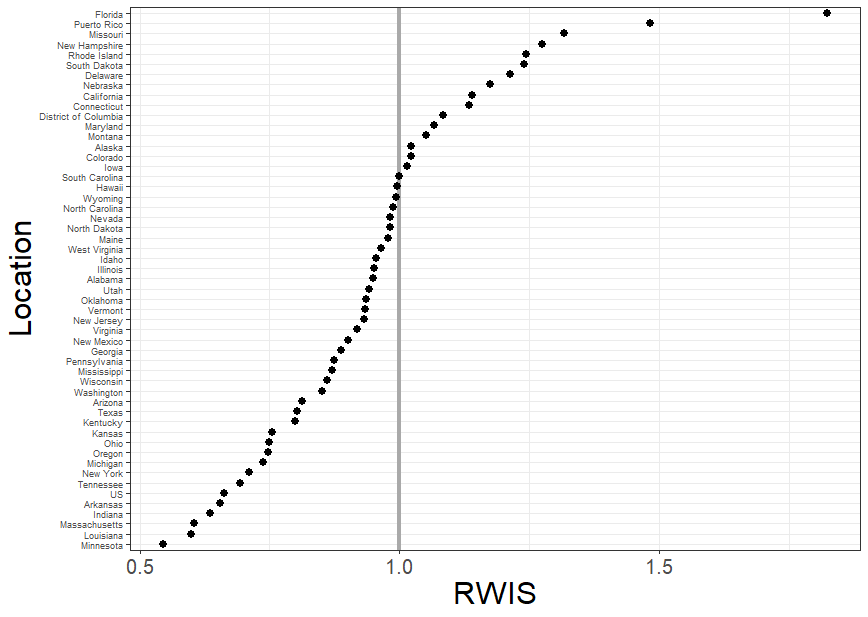
\includegraphics[scale=.5]{Images/sir_disc_hosp_sq_ar1_rwis.png}
%     \caption{Overall median RWIS by location (black points) for forecasts made by a model including the SIR model with discrepancy, the normal hospitalization model with the square ILI term. The grey line at RWIS = 1 represents the RWIS for the baseline forecast.}
%     \label{fig:sir_disc_sq_rwis}
% \end{figure}


% \subsection{Model Comparison}

% Here the quantile forecasts of our models are compared with those of 10 teams who submitted forecasts during the 2023 flu season. The forecasts selected for comparison were chosen based on similarities shared with our in terms of data and methods used. The FluSight-baseline and FluSight-ensemble models are also included in the comparison. The table below summarizes the information for the selected models and is populated with information given by the forecast teams with their submissions (??). 

% \begin{table}[htbp]
%     \centering
%     \begin{tabular}{ |p{3cm}||p{2.8cm}|p{6cm}|p{1.6cm}|  }
%          \hline
%          Model name & Additional Data & Model Summary & Ensemble\\
%          \hline
%          CU-ensemble  & ILI & Ensemble of mechanistic and statistical models& Yes\\
%          \hline
%          LosAlamos\_NAU &  & Bayesian Compartmental & No\\
%          \hline
%          MOBS &  & Metapopulation "SLIR" & No\\
%          \hline
%          UGA\_flucast-Copycat & ILIp, FluServ & Pattern matching/Nearest neighbor & No\\
%          \hline
%          UM-DeepOutbreak & Google symptom search data, ILI & Deep neural network & No\\
%          \hline
%          UMass-flusion & Flu\_Surv, ILI, WHO/NREVSS test & Ensemble of statistical/machine learning time series & Yes\\
%          \hline
%     \end{tabular}
%     \caption{Caption}
%     \label{tab:my_label}
% \end{table}

% The overall forecasts are compared visually using PIT histograms (??) and reliability diagrams (??). These plots are used to assess model calibration, which in probabilistic forecasting relies on the...




\section{Conclusion}
\label{sec:conclusion}

 In this manuscript we introduce a statistical modeling framework which allows for the incorporation of several ILI forecast modeling methods. Specifically, we built upon \cite{osthus2019dynamic} and introduced a framework for modeling ILI which includes the use of an arbitrary function for modeling the main trajectory of ILI along with modeling the discrepancy. We model flu hospitalizations by incorporating the ILI forecast model into a model forecasting hospitalizations where hospitalization predictions are a linear or quadratic function of ILI.

The simulation study in section \ref{sec:simulation2} suggests the ASG function in ILI modeling may slightly outperform the SIR model according to the LogS and CRPS scoring rules, but in the analysis of the 2023 flu season forecasts, the SIR model was overall superior. The results from both the simulation study and the real data analysis suggest that the addition of a discrepancy component in ILI modeling may improve forecasts especially near the holiday week between Christmas and New Years day. It should not be assumed that these conclusions may be generalized for all locations in the US, weeks of a season, or for future flu seasons. 
% Rather than deciding to use or not to use certain of the modeling techniques here, a more promising option may be to combine forecasts from various models into an ensemble forecast. 

Forecasting the seasonal influenza outbreak remains a challenging task for forecasters. The general modeling framework in this manuscript is successful under diverse modeling conditions for all locations in the US and may contribute to future forecasting efforts. All forecast models were presented as separate from one another, but in the various locations and times of the flu season, different models perform better than others. To build on the work done here, a natural step forward would be to combine all or a few selected forecasts into an ensemble forecast. Such an ensemble may work to cancel out certain model biases or highlight model strengths, leading to more robust forecasts. 


\section{Acknowledgments}
This work is partially supported by the National Science Foundation under Grant No. 2152117. Any opinions, findings, and conclusions or recommendations expressed in this material are those of the author(s) and do not necessarily reflect the views of the National Science Foundation.
% \spencer{I noticed that Luis acknowledged HPC@ISU for his work. Should I do the same?}

%%%%%%%%

%%%%
% Reference section comes before the appendix

%\bibliographystyle{acm} % use for numbered citations along with options given in preamble. Look at the main thesis.tex file
\bibliographystyle{apa}

\bibliography{master_bib}

% %\section{Bibliography}
% \bibliographystyle{apa}
% % \vspace{-20pt}
% \begingroup
%     \setlength{\bibsep}{13.2pt}
%     \linespread{1}\selectfont
%     \bibliography{master_bib}
% \endgroup
% \clearpage
% \pagebreak

%%%%%
%% Appendix
% This section may or may not be included
% Chapter 2 shows a double appendix example. Please use A or B as in Appendix A if there are multiple appendix. Use "Appendix A:" before writing the title
% Chapter 3 shows a single appendix example. Use "Appendix:" before writing the title 

\begin{appendices}
\section{FluSight forecast competition scoring results} \label{app:A_rwis}

In the CDC flu forecast competition, a baseline forecast was made to which all other forecasts were compared. The baseline forecast for a given state and week had as a median the most recent observed hospitalization count. The uncertainty was based on differences between previous hospitalizations, and is similar to the baseline forecast used in previous flu forecasting seasons and in the COVID-19 hub \cite[]{mathis2024evaluation, cramer2022evaluation}. 
The RWIS for one model was calculated by first taking the ratio of the average LWIS paired with every other model. This was then diveded by the same ratio for the baseline forecasts (see methods in \cite{mathis2024evaluation} for details, and see also the supplementary material).
 An RWIS less than 1 indicates the forecast outperformed the baseline forecast.
 Figures \ref{fig:rwis_ili_tile} and \ref{fig:rwis_hosp_tile} show the mean RWIS of hospitalization forecasts over all 24 models from section \ref{sec:analysis} for all locations and weeks of the 2023 flu season. Some similar patterns to those noted in section \ref{sec:analysis} emerge, including a slightly better performance by forecasts including discrepancy modeling over those which do not include discrepancy modeling and better overall performance by the SIR models than by the ASG forecast models. Interestingly, figure \ref{fig:rwis_hosp_tile} shows the LNORM model showing especially poor RWIS performance about three quarters into the season. This was not seen in the LWIS in figure \ref{fig:lwis_by_dist_loc}. 


\begin{figure}
    \centering
    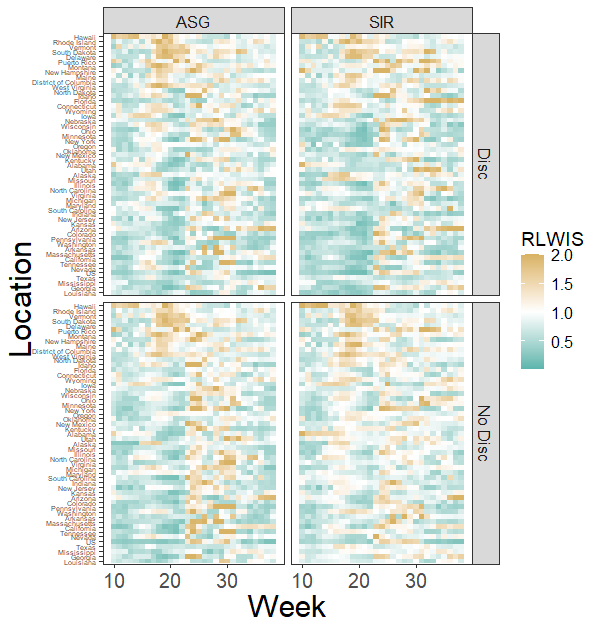
\includegraphics[scale=.7]{Images/rwis_ili_mod.png}
    \caption{RWIS averaged over all 24 models and horizons for forecasts across all locations and weeks. The plot is separated by the four ILI models. Dark blue is lower RWIS, and dark tan is higher RWIS where white is RWIS = 1}
    \label{fig:rwis_ili_tile}
\end{figure}


\begin{figure}
    \centering
    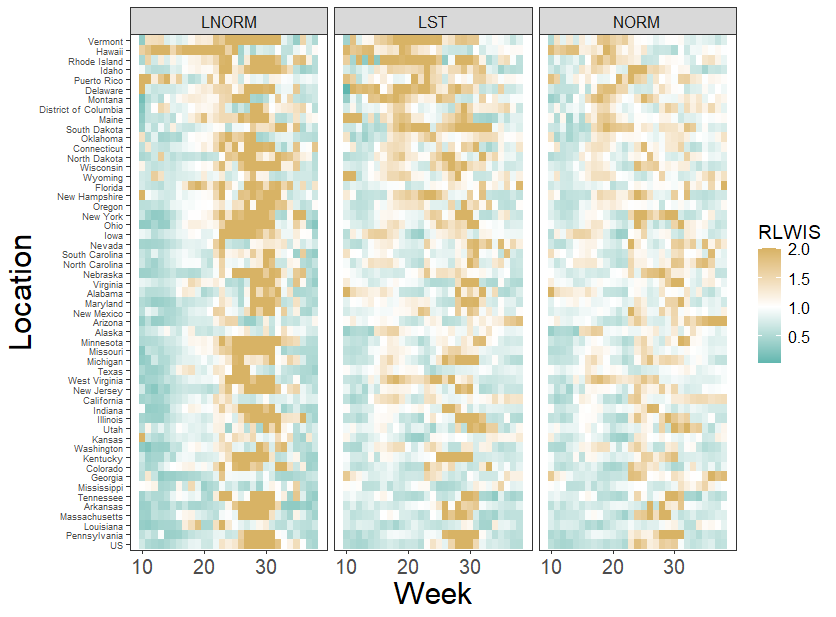
\includegraphics[scale=.6]{Images/rwis_hosp_mod.png}
    \caption{RWIS averaged over all 24 models and horizons for forecasts across all locations and weeks. The plot is separated by the three distribution choices for the hospitalization model. Dark blue is lower RWIS, and dark tan is higher RWIS where white is RWIS = 1}
    \label{fig:rwis_hosp_tile}
\end{figure}


Figure \ref{fig:state_median_points} shows the mean over weeks RWIS for the SIR and ASG forecast models with an RWIS less than 1 for the most locations. The plot on the left is from a forecast by an SIRD ILI model and a quadratic NORM hospitalization model. This forecast model had an RWIS less than 1 for 37 out of 53 locations. The plot on the right is from a forecast by an ASGD ILI model and linear NORM hospitalization model. This model had an RWIS less than 1 for 34 out of 53 locations.

\begin{figure}
\centering
\begin{subfigure}{.5\textwidth}
  \centering
  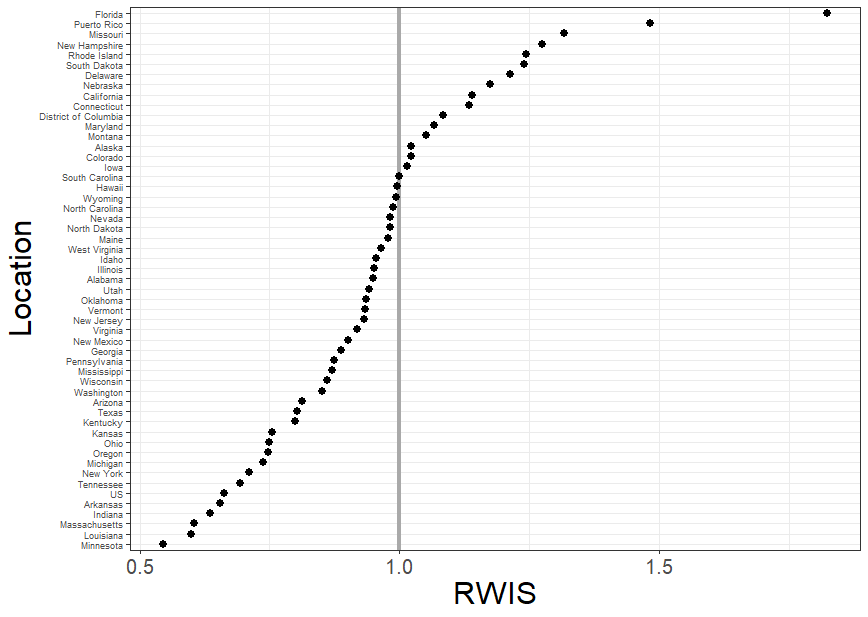
\includegraphics[width=1\linewidth]{Images/sir_disc_hosp_sq_ar1_rwis.png}
  % \caption{A subfigure}
  % \label{fig:sub1}
\end{subfigure}%
\begin{subfigure}{.5\textwidth}
  \centering
  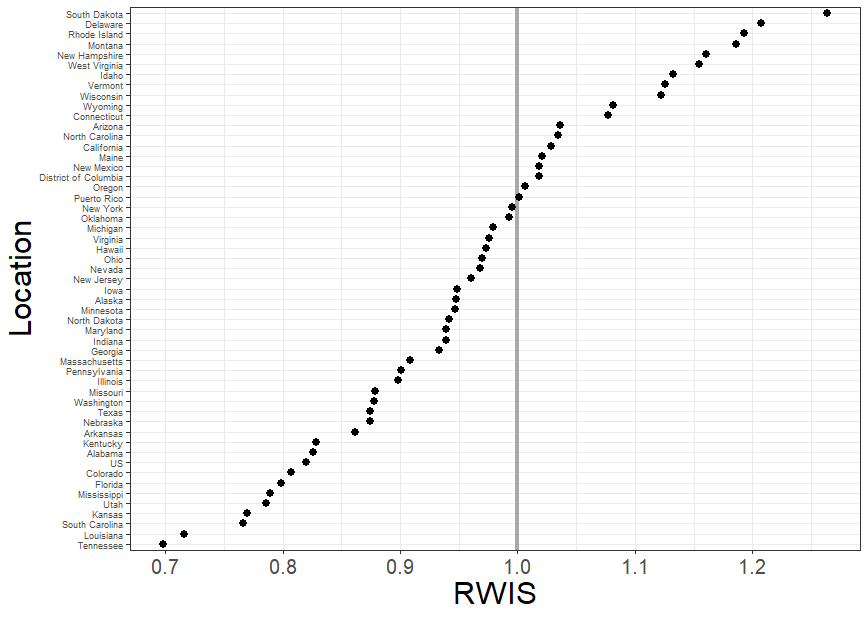
\includegraphics[width=1\linewidth]{Images/asg_disc_hosp_ar1_rwis.png}
  % \caption{A subfigure}
  % \label{fig:sub2}
\end{subfigure}
\caption{RWIS over the whole 2023 flu season for all 53 locations for hospitalization forecasts from an SIRD quadratic hospitalization model with normal errors (left) and forecasts from an ASGD linear hospitalization model with normal errors (right). An RWIS less than 1 (left of vertical grey line) indicates the model forecasts outperformed the baseline forecasts for that particular region.}
\label{fig:state_median_points}
\end{figure}






\section{Posterior distribution plots for select parameters}
\label{app:B_prior}

The figures in this section show 95\% credible intervals for model parameters under the several modeling schemes along with the prior distributions assigned to the parameters. Figure \ref{fig:posterior_theta_sir} is for parameters unique to the SIR ILI model. Figures \ref{fig:posterior_theta} and \ref{fig:posterior_zeta} are for parameters unique to the ASG models. Figure \ref{fig:sir_asg_shared} is for parameters shared by SIR and ASG models, including parameters used for modeling discrepancy. Figures \ref{fig:hosp_lin_params} and \ref{fig:hosp_nus_param} are for parameters used in hospitalization modeling.


\begin{figure}
    \centering
    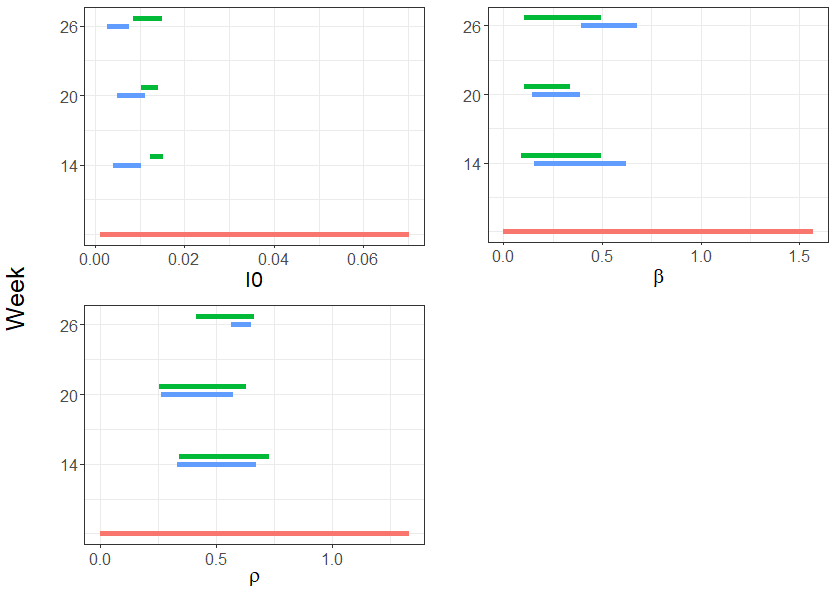
\includegraphics[scale=.6]{Images/posterior_theta_sir.png}
    \caption{Posterior 95\% credible intervals from ILI model for parameters of SIR differential equations. Shown are intervals from the US model of ILI for weeks 14, 20, and 26. The green is from the posterior where discrepancy is not modeled, and the blue is from the model where it is. The red interval is the 95\% interval of the prior distribution.}
    \label{fig:posterior_theta_sir}
\end{figure}

\begin{figure}
    \centering
    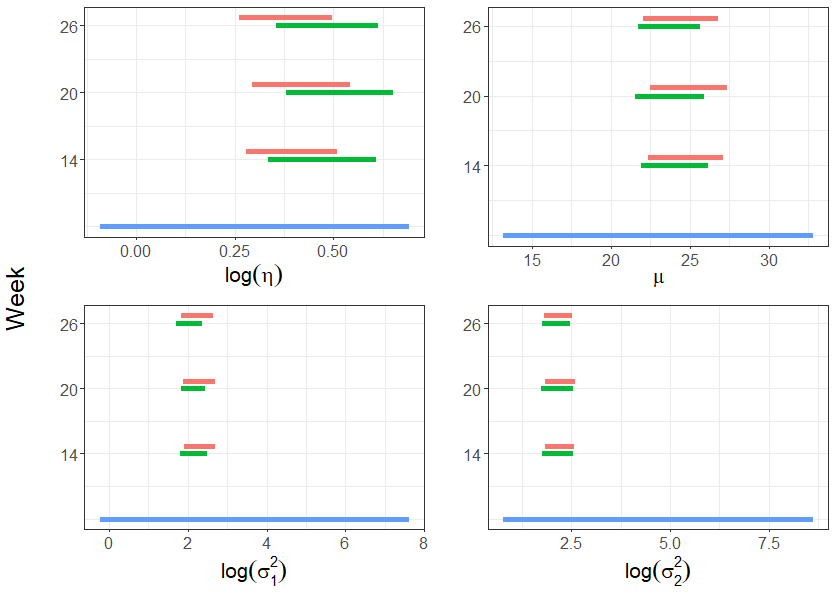
\includegraphics[scale=.6]{Images/posterior_theta.png}
    \caption{Posterior 95\% credible intervals from ILI model for parameters of ASG function. Shown are intervals from the US model of ILI for weeks 14, 20, and 26. The red is from the posterior where discrepancy is not modeled, and the green is from the model where it is. The blue interval is the 95\% interval of the prior distribution.}
    \label{fig:posterior_theta}
\end{figure}


\begin{figure}
    \centering
    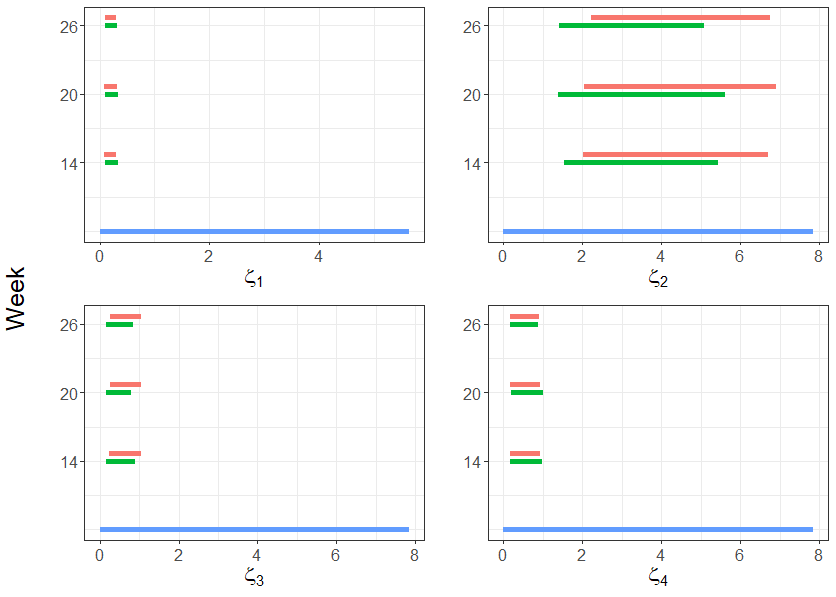
\includegraphics[scale=.6]{Images/posterior_zeta.png}
    \caption{Posterior 95\% credible intervals from ILI model for variance parameters of the ASG function. Shown are intervals from the US model of ILI for weeks 14, 20, and 26. The red is from the posterior where discrepancy is not modeled, and the green is from the model where it is. The blue interval is the 95\% interval of the prior distribution.}
    \label{fig:posterior_zeta}
\end{figure}

\begin{figure}
\centering
\begin{subfigure}{.5\textwidth}
  \centering
  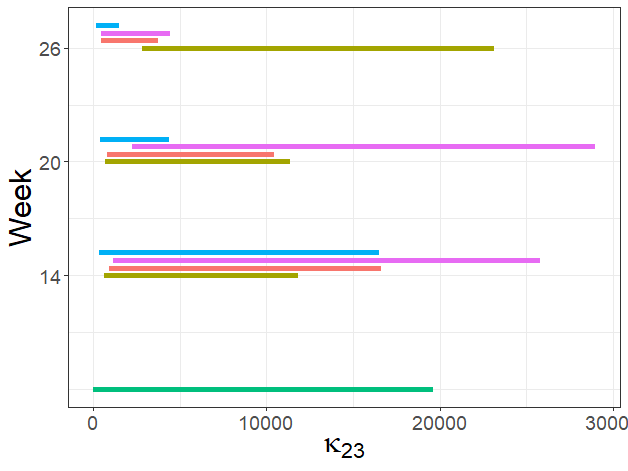
\includegraphics[width=.8\linewidth]{Images/posterior_kappa.png}
  % \caption{95\% posterior credible intervals from ILI model for scale parameter of the model distribution. Shown are intervals from the US model of ILI for weeks 14, 20, and 26. The blue is from the SIR model, purple from SIRD, red from ASG and yellow from ASGD. The green interval is the 95\% interval of the prior distribution.}
  % \label{fig:sub1}
\end{subfigure}%
\begin{subfigure}{.5\textwidth}
  \centering
  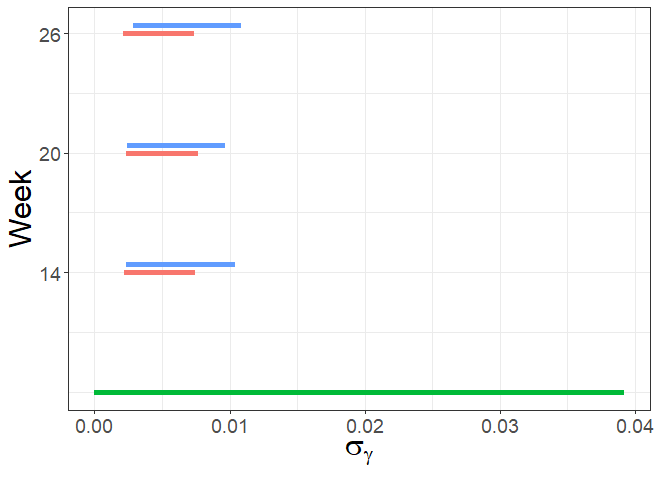
\includegraphics[width=.8\linewidth]{Images/posterior_sigma_gamma.png}
  % \caption{95\% posterior credible intervals from ILI model for scale parameter of modeled discrepancy. Shown are intervals from the US model of ILI for weeks 14, 20, and 26. The blue is from the SIRD model and red from ASGD. The green interval is the 95\% interval of the prior distribution.}
  % \label{fig:sub2}
\end{subfigure}
\caption{Posterior 95\% credible intervals from ILI model for scale parameter $\kappa_s$. Blue is from the SIR model, purple from SIRD, red from ASG and yellow from ASGD (left).  Posterior 95\% credible intervals from ILI model for scale parameter of modeled discrepancy $\sigma_{\gamma}$ (right). Shown are intervals from the US model of ILI for weeks 14, 20, and 26. Blue is from the SIRD model and red from ASGD. The green interval is the 95\% interval of the prior distribution.}
\label{fig:sir_asg_shared}
\end{figure}

\begin{figure}[hbt!]

\begin{subfigure}{.475\linewidth}
  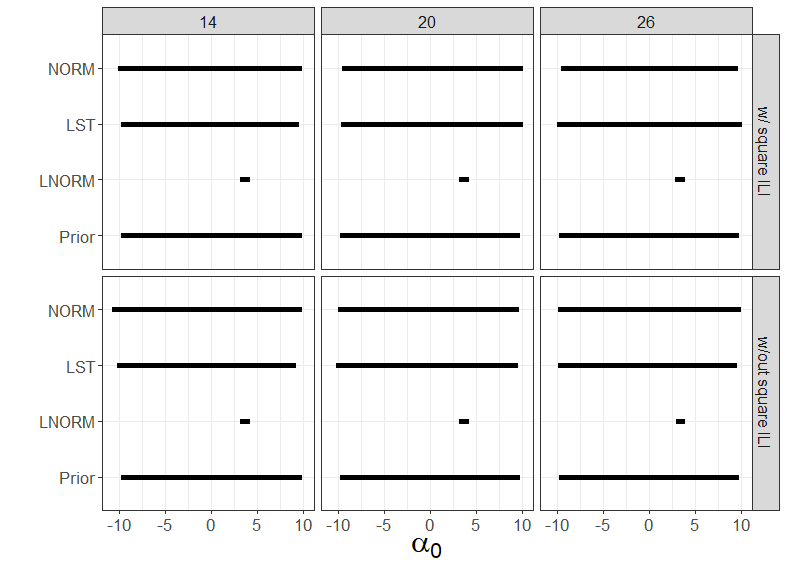
\includegraphics[width=\linewidth]{Images/alpha0_post.png}
  % \caption{}
  % \label{MLEDdet}
\end{subfigure}\hfill % <-- "\hfill"
\begin{subfigure}{.475\linewidth}
  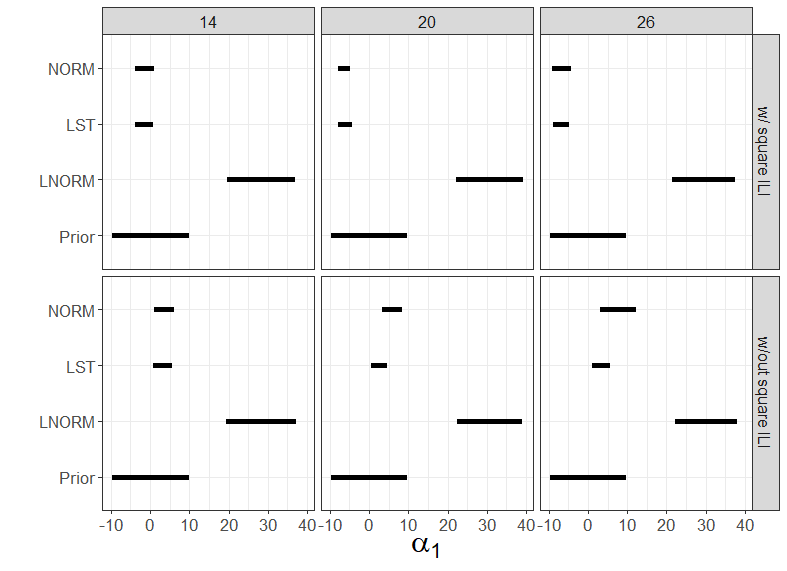
\includegraphics[width=\linewidth]{Images/alpha1_post.png}
  % \caption{}
  % \label{energydetPSK}
\end{subfigure}

\medskip % create some *vertical* separation between the graphs
\begin{subfigure}{.475\linewidth}
  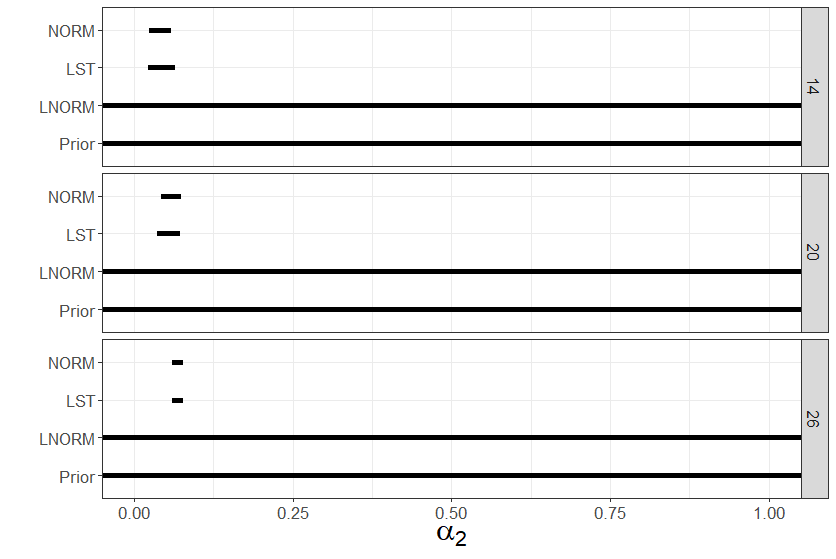
\includegraphics[width=\linewidth]{Images/alpha2_post.png}
  % \caption{}
  % \label{velcomp}
\end{subfigure}\hfill % <-- "\hfill"
\begin{subfigure}{.475\linewidth}
  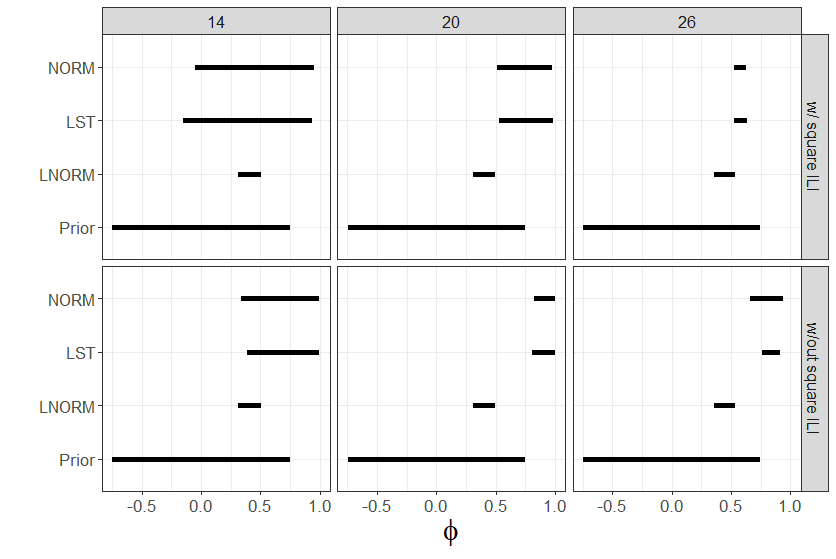
\includegraphics[width=\linewidth]{Images/phi_post.png}
  % \caption{}
  % \label{estcomp}
\end{subfigure}

\caption{Posterior 95\% credible intervals for $\alpha_0$ for the three hospitalization models separated by whether or not the squared ILI term was included. Intervals are for the US hospitalizations and weeks 14, 20 and 26 are shown (top left). Prior distribution 95\% interval is also included.  95\% posterior credible intervals for $\alpha_1$ for the three hospitalization models separated by whether or not the squared ILI term was included. Intervals are for the US hospitalizations and weeks 14, 20 and 26 are shown (top right). Prior distribution 95\% interval is also included.
95\% posterior credible intervals for $\alpha_2$ for the three hospitalization models. Intervals are for the US hospitalizations and weeks 14, 20 and 26 are shown (bottom left). Prior distribution 95\% interval is also included. 
95\% posterior credible intervals for $\phi$ for the three hospitalization models separated by whether or not the squared ILI term was included (bottom right). Prior distribution 95\% interval is also included. In each plot intervals are for the US hospitalizations and weeks 14, 20 and 26 are shown.}
\label{fig:hosp_lin_params}
\end{figure}


\begin{figure}[hbt!]

\begin{subfigure}{.475\linewidth}
  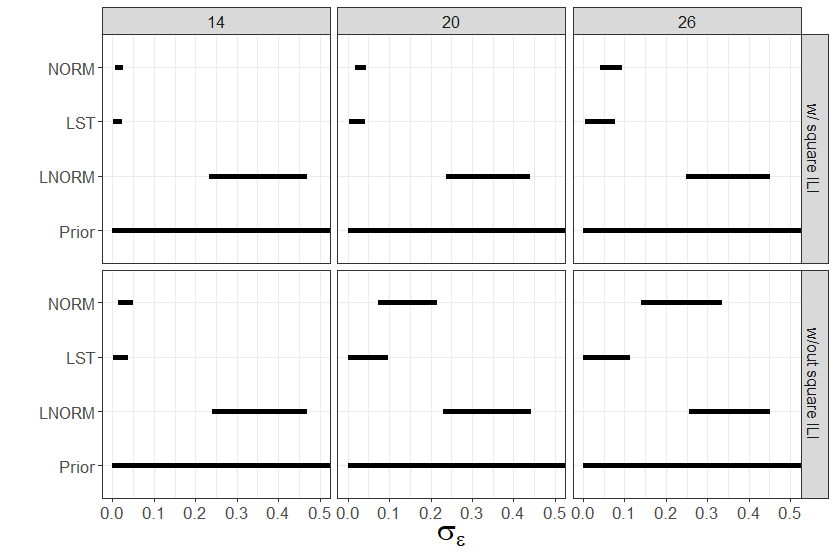
\includegraphics[width=\linewidth]{Images/sigma_epsilon_post.png}
  % \caption{}
  % \label{MLEDdet}
\end{subfigure}\hfill % <-- "\hfill"
\begin{subfigure}{.475\linewidth}
  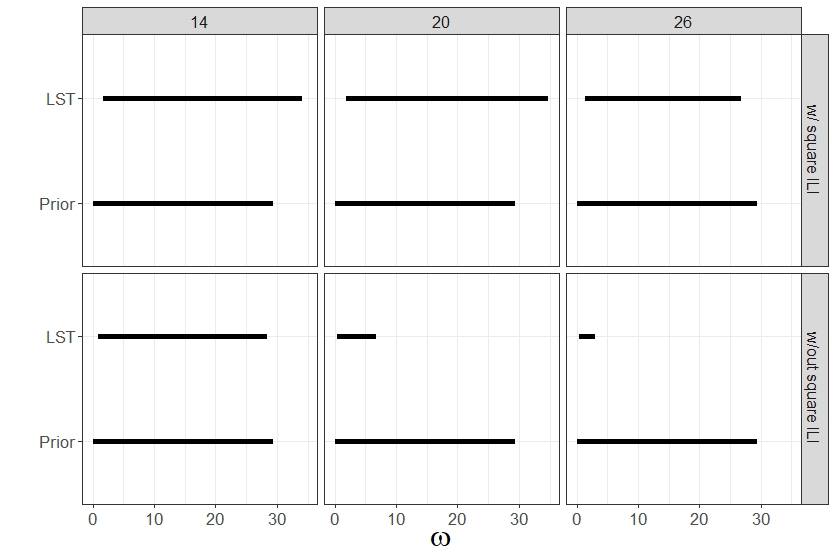
\includegraphics[width=\linewidth]{Images/omega_post.png}
  % \caption{}
  % \label{energydetPSK}
\end{subfigure}

\caption{Posterior 95\% credible intervals for $\sigma_{\epsilon}$ for hospitalization models with and without the ILI squared term. Intervals are for the US hospitalizations and weeks 14, 20 and 26 are shown (left). Prior distribution 95\% interval is also included.
95\% posterior credible intervals for $\omega$ for LST hospitalization models with and without the ILI squared term (right). Prior distribution 95\% interval is also included. In all plots intervals are for the US hospitalizations and weeks 14, 20 and 26 are shown.}
\label{fig:hosp_nus_param}
\end{figure}



% \begin{figure}
% \centering
% \begin{subfigure}{.5\textwidth}
%   \centering
%   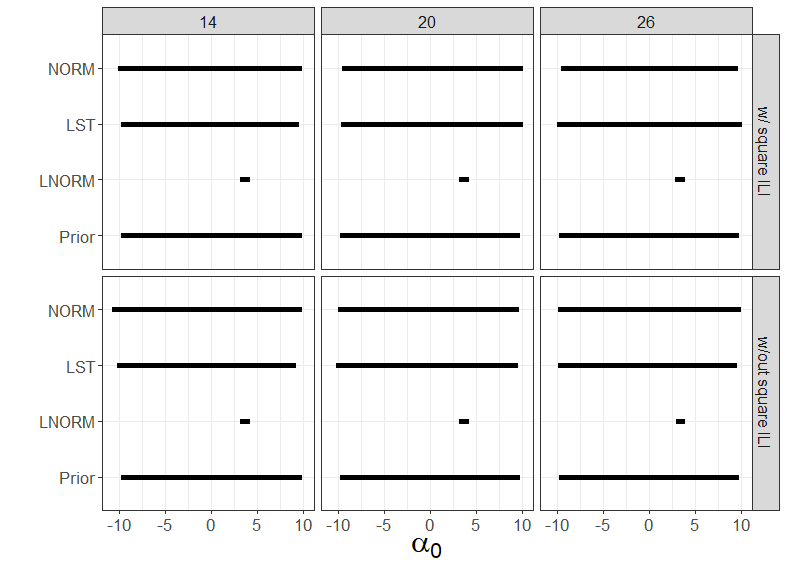
\includegraphics[width=.8\linewidth]{Images/alpha0_post.png}
% \end{subfigure}%
% \begin{subfigure}{.5\textwidth}
%   \centering
%   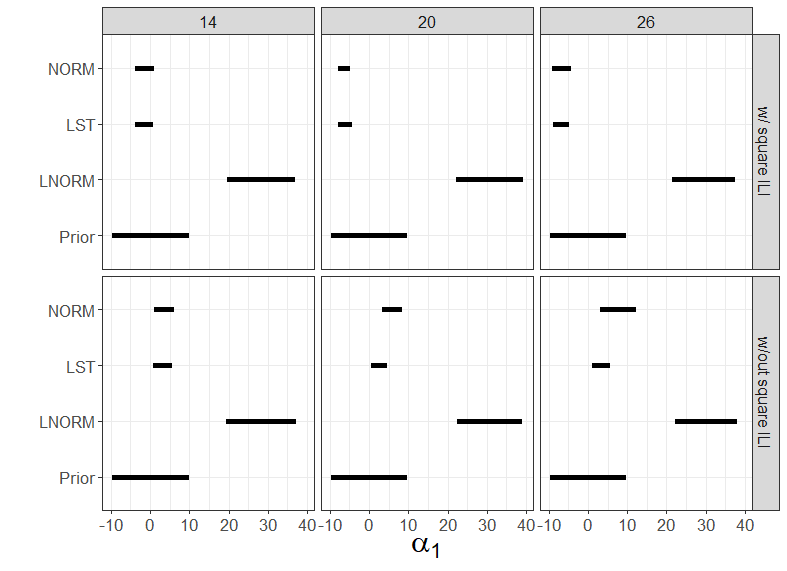
\includegraphics[width=.8\linewidth]{Images/alpha1_post.png}
% \end{subfigure}
% \caption{(left) 95\% posterior credible intervals for $\alpha_0$ for the three hospitalization models separated by whether or not the squared ILI term was included. Intervals are for the US hospitalizations and weeks 14, 20 and 26 are shown. Prior distribution 95\% interval is also included. (right) 95\% posterior credible intervals for $\alpha_1$ for the three hospitalization models separated by whether or not the squared ILI term was included. Intervals are for the US hospitalizations and weeks 14, 20 and 26 are shown. Prior distribution 95\% interval is also included.}
% \label{fig:hosp_params_post1}
% \end{figure}

% \begin{figure}
%     \centering
%     \includegraphics[scale=.5]{Images/alpha0_post.png}
%     \caption{95\% posterior credible intervals for $\alpha_0$ for the three hospitalization models separated by whether or not the squared ILI term was included. Intervals are for the US hospitalizations and weeks 14, 20 and 26 are shown. 95\% interval for prior distribution is also included}
%     \label{fig:alpha0_post}
% \end{figure}


% \begin{figure}
%     \centering
%     \includegraphics[scale=.6]{Images/alpha1_post.png}
%     \caption{95\% posterior credible intervals for $\alpha_1$ for the three hospitalization models separated by whether or not the squared ILI term was included. Intervals are for the US hospitalizations and weeks 14, 20 and 26 are shown. 95\% interval for prior distribution is also included}
%     \label{fig:alpha1_post}
% \end{figure}


% \begin{figure}
% \centering
% \begin{subfigure}{.5\textwidth}
%   \centering
%   \includegraphics[width=.8\linewidth]{Images/alpha2_post.png}
%   % \caption{95\% posterior credible intervals from ILI model for scale parameter of the model distribution. Shown are intervals from the US model of ILI for weeks 14, 20, and 26. The blue is from the SIR model, purple from SIRD, red from ASG and yellow from ASGD. The green interval is the 95\% interval of the prior distribution.}
%   % \label{fig:sub1}
% \end{subfigure}%
% \begin{subfigure}{.5\textwidth}
%   \centering
%   \includegraphics[width=.8\linewidth]{Images/phi_post.png}
  
%   % \label{fig:sub2}
% \end{subfigure}

% \begin{subfigure}{.5\textwidth}
%   \centering
%   \includegraphics[width=.8\linewidth]{Images/omega_post.png}

  
  
%   % \label{fig:sub2}
  
% \end{subfigure}
% \begin{subfigure}{.5\textwidth}
%   \centering
%   \includegraphics[width=.8\linewidth]{Images/sigma_epsilon_post.png}
% \end{subfigure}
% \caption{(top left) 95\% posterior credible intervals for $\alpha_2$ for the three hospitalization models. Intervals are for the US hospitalizations and weeks 14, 20 and 26 are shown. Prior distribution 95\% interval is also included. 
% (top right) 95\% posterior credible intervals for $\phi$ for the three hospitalization models separated by whether or not the squared ILI term was included. Intervals are for the US hospitalizations and weeks 14, 20 and 26 are shown. Prior distribution 95\% interval is also included. (bottom) 95\% posterior credible intervals for $\omega$ for LST hospitalization models with and without the ILI squared term. Intervals are for the US hospitalizations and weeks 14, 20 and 26 are shown. 95\% interval for prior distribution is also included}
% \label{fig:hosp_params_post2}
% \end{figure}


% \begin{figure}[hbt!]

% \begin{subfigure}{.475\linewidth}
%   \includegraphics[width=\linewidth]{Images/alpha0_post.png}
%   % \caption{}
%   % \label{MLEDdet}
% \end{subfigure}\hfill % <-- "\hfill"
% \begin{subfigure}{.475\linewidth}
%   \includegraphics[width=\linewidth]{Images/alpha1_post.png}
%   % \caption{}
%   % \label{energydetPSK}
% \end{subfigure}

% \medskip % create some *vertical* separation between the graphs
% \begin{subfigure}{.475\linewidth}
%   \includegraphics[width=\linewidth]{Images/alpha2_post.png}
%   % \caption{}
%   % \label{velcomp}
% \end{subfigure}\hfill % <-- "\hfill"
% \begin{subfigure}{.475\linewidth}
%   \includegraphics[width=\linewidth]{Images/phi_post.png}
%   % \caption{}
%   % \label{estcomp}
% \end{subfigure}

% \caption{A figure with four subfigures}
% \label{fig:roc}
% \end{figure}

% \begin{figure}
%     \centering
%     \includegraphics[scale=.6]{Images/alpha2_post.png}
%     \caption{95\% posterior credible intervals for $\alpha_2$ for the three hospitalization models. Intervals are for the US hospitalizations and weeks 14, 20 and 26 are shown. 95\% interval for prior distribution is also included}
%     \label{fig:alpha2_post}
% \end{figure}


% \begin{figure}
%     \centering
%     \includegraphics[scale=.6]{Images/phi_post.png}
%     \caption{95\% posterior credible intervals for $\phi$ for the three hospitalization models separated by whether or not the squared ILI term was included. Intervals are for the US hospitalizations and weeks 14, 20 and 26 are shown. 95\% interval for prior distribution is also included}
%     \label{fig:phi_post}
% \end{figure}


% \begin{figure}
%     \centering
%     \includegraphics[scale=.]{Images/omega_post.png}
%     \caption{95\% posterior credible intervals for $\omega$ for LST hospitalization models with and without the ILI squared term. Intervals are for the US hospitalizations and weeks 14, 20 and 26 are shown. 95\% interval for prior distribution is also included}
%     \label{fig:omega_post}
% \end{figure}


% This section may or may not be included
% \newpage
% \section{Appendix B: Additional tables showing median RWIS for location-model combinations}
% \label{app:B_tables}


% \begin{table}

% % \parbox{.45\linewidth}{
% \raggedleft
% \caption{Model with minimum median RWIS by location}
% \small
% \centering
% \begin{tabular}[t]{rrr}
% \label{tab:wis_by_state}
% \textbf{Location} & \textbf{Model} & \textbf{RWIS}\\

% Alabama & ASGD-NORM & 0.768\\

% Alaska & ASG-NORM-SQ & 0.886\\

% Arizona & ASG-NORM-SQ & 0.669\\

% Arkansas & SIRD-NORM-SQ & 0.734\\

% California & ASGD-NORM-SQ & 0.688\\

% Colorado & SIRD-NORM & 0.619\\

% Connecticut & ASG-NORM & 0.945\\

% Delaware & SIR-NORM-SQ & 0.836\\

% District of Columbia & ASGD-LST-SQ & 0.970\\

% Florida & ASGD-NORM-SQ & 0.680\\

% Georgia & ASG-LNORM & 0.595\\

% Hawaii & SIRD-LST & 0.979\\

% Idaho & ASGD-NORM & 0.895\\

% Illinois & SIRD-LST-SQ & 0.757\\

% Indiana & SIRD-NORM-SQ & 0.696\\

% Iowa & ASGD-NORM & 0.948\\

% Kansas & ASG-NORM-SQ & 0.753\\

% Kentucky & ASG-NORM-SQ & 0.697\\

% Louisiana & SIRD-LST & 0.533\\

% Maine & ASG-NORM-SQ & 0.879\\

% Maryland & SIRD-LNORM & 0.737\\

% Massachusetts & SIRD-NORM-SQ & 0.632\\

% Michigan & SIRD-LST-SQ & 0.733\\

% Minnesota & SIRD-LST-SQ & 0.673\\

% Mississippi & SIR-LNORM-SQ & 0.742\\

% Missouri & ASG-NORM-SQ & 0.797\\

% Montana & SIRD-LNORM-SQ & 0.855\\

% Nebraska & ASGD-NORM-SQ & 0.934\\

% Nevada & SIRD-NORM-SQ & 0.786\\

% New Hampshire & SIR-NORM & 0.766\\

% New Jersey & ASG-LST & 0.811\\

% New Mexico & SIRD-LNORM & 0.768\\

% New York & SIRD-NORM-SQ & 0.765\\

% North Carolina & ASGD-LST & 0.818\\

% North Dakota & ASG-NORM-SQ & 0.838\\

% Ohio & SIRD-NORM & 0.803\\

% Oklahoma & ASGD-NORM-SQ & 0.861\\

% Oregon & SIRD-LST & 0.838\\

% Pennsylvania & SIRD-LNORM & 0.725\\

% Puerto Rico & SIRD-LST & 0.966\\

% Rhode Island & ASG-NORM & 0.869\\

% South Carolina & ASG-LST & 0.670\\

% South Dakota & SIR-LNORM & 0.950\\

% Tennessee & ASG-LST & 0.610\\

% Texas & SIRD-LST-SQ & 0.737\\

% US & ASG-LST-SQ & 0.563\\


% Utah & ASG-LST & 0.702\\

% Vermont & SIRD-NORM-SQ & 0.960\\

% Virginia & ASG-LST & 0.828\\

% Washington & SIRD-NORM & 0.753\\

% West Virginia & SIRD-LNORM & 0.828\\

% Wisconsin & SIRD-LST-SQ & 0.793\\

% Wyoming & SIRD-LNORM & 0.836\\
% \hline
% \end{tabular}
% % \end{table}
% % }
% \end{table}

% \begin{table}
% \hfill
% % \parbox{.45\linewidth}{
% % \begin{table}
% % \raggedright
% \caption{Overall median RWIS and WIS by model}
% \small
% \centering
% \begin{tabular}[t]{c|cc}
% \label{tab:wis_by_model}
% \textbf{Model} & \textbf{RWIS} & \textbf{WIS}\\
% \hline
% SIRD-NORM-SQ & 0.898 & 15.884\\

% ASG-NORM-SQ & 0.903 & 17.152\\

% ASGD-NORM-SQ & 0.922 & 17.408\\

% SIRD-LST-SQ & 0.926 & 16.806\\

% SIRD-NORM & 0.928 & 16.371\\

% ASG-LST-SQ & 0.934 & 18.116\\

% ASGD-LST-SQ & 0.943 & 17.949\\

% SIRD-LST & 0.943 & 17.113\\

% SIRD-LNORM & 0.945 & 20.046\\

% ASG-NORM & 0.946 & 16.762\\

% SIRD-LNORM-SQ & 0.951 & 20.110\\

% ASG-LST & 0.957 & 17.180\\

% ASGD-NORM & 0.966 & 17.208\\

% ASGD-LST & 0.968 & 17.487\\

% ASG-LNORM & 0.968 & 20.628\\

% ASG-LNORM-SQ & 0.969 & 20.620\\

% ASGD-LNORM & 0.982 & 21.108\\

% ASGD-LNORM-SQ & 0.986 & 20.992\\

% FluSight-baseline & 1.000 & 17.585\\

% SIR-NORM-SQ & 1.002 & 18.156\\

% SIR-LNORM & 1.009 & 21.441\\

% SIR-LST-SQ & 1.009 & 18.547\\

% SIR-LNORM-SQ & 1.013 & 21.494\\

% SIR-LST & 1.034 & 19.000\\

% SIR-NORM & 1.067 & 19.904\\
% \hline
% \end{tabular}
% % }
% \end{table}

\end{appendices}